% ****** Start of file apssamp.tex ******
%DIF LATEXDIFF DIFFERENCE FILE
%DIF DEL main_20260529.tex   Fri Jun  5 19:24:44 2026
%DIF ADD main.tex            Fri Jun  5 20:10:03 2026
%
%   This file is part of the APS files in the REVTeX 4.2 distribution.
%   Version 4.2a of REVTeX, December 2014
%
%   Copyright (c) 2014 The American Physical Society.
%
%   See the REVTeX 4 README file for restrictions and more information.
%
% TeX'ing this file requires that you have AMS-LaTeX 2.0 installed
% as well as the rest of the prerequisites for REVTeX 4.2
%
% See the REVTeX 4 README file
% It also requires running BibTeX. The commands are as follows:
%
%  1)  latex apssamp.tex
%  2)  bibtex apssamp
%  3)  latex apssamp.tex
%  4)  latex apssamp.tex
%
\documentclass[%
 reprint,
superscriptaddress,
%groupedaddress,
%unsortedaddress,
%runinaddress,
%frontmatterverbose,
%preprint,
%preprintnumbers,
%nofootinbib,
%nobibnotes,
%bibnotes,
 amsmath,amssymb,
 aps,
%pra,
%prb,
%rmp,
%prstab,
%prstper,
%floatfix,
]{revtex4-2}

\usepackage{graphicx}% Include figure files
\usepackage{dcolumn}% Align table columns on decimal point
\usepackage{bm}% bold math
\usepackage{comment}
% \usepackage{luatexja}
\usepackage{enumitem}
\usepackage[version=4]{mhchem}
\usepackage[hidelinks]{hyperref}% add hypertext capabilities
%\usepackage[mathlines]{lineno}% Enable numbering of text and display math
%\linenumbers\relax % Commence numbering lines

%\usepackage[showframe,%Uncomment any one of the following lines to test
%%scale=0.7, marginratio={1:1, 2:3}, ignoreall,% default settings
%%text={7in,10in},centering,
%%margin=1.5in,
%%total={6.5in,8.75in}, top=1.2in, left=0.9in, includefoot,
%%height=10in,a5paper,hmargin={3cm,0.8in},
%]{geometry}
\newcommand{\He}{$^3$He }
\newcommand{\Hensf}{$^3$He-NSF}
%DIF PREAMBLE EXTENSION ADDED BY LATEXDIFF
%DIF UNDERLINE PREAMBLE %DIF PREAMBLE
\RequirePackage[normalem]{ulem} %DIF PREAMBLE
\RequirePackage{color}\definecolor{RED}{rgb}{1,0,0}\definecolor{BLUE}{rgb}{0,0,1} %DIF PREAMBLE
\providecommand{\DIFaddtex}[1]{{\protect\color{blue}\uwave{#1}}} %DIF PREAMBLE
\providecommand{\DIFdeltex}[1]{{\protect\color{red}\sout{#1}}}                      %DIF PREAMBLE
%DIF SAFE PREAMBLE %DIF PREAMBLE
\providecommand{\DIFaddbegin}{} %DIF PREAMBLE
\providecommand{\DIFaddend}{} %DIF PREAMBLE
\providecommand{\DIFdelbegin}{} %DIF PREAMBLE
\providecommand{\DIFdelend}{} %DIF PREAMBLE
\providecommand{\DIFmodbegin}{} %DIF PREAMBLE
\providecommand{\DIFmodend}{} %DIF PREAMBLE
%DIF FLOATSAFE PREAMBLE %DIF PREAMBLE
\providecommand{\DIFaddFL}[1]{\DIFadd{#1}} %DIF PREAMBLE
\providecommand{\DIFdelFL}[1]{\DIFdel{#1}} %DIF PREAMBLE
\providecommand{\DIFaddbeginFL}{} %DIF PREAMBLE
\providecommand{\DIFaddendFL}{} %DIF PREAMBLE
\providecommand{\DIFdelbeginFL}{} %DIF PREAMBLE
\providecommand{\DIFdelendFL}{} %DIF PREAMBLE
%DIF HYPERREF PREAMBLE %DIF PREAMBLE
\providecommand{\DIFadd}[1]{\texorpdfstring{\DIFaddtex{#1}}{#1}} %DIF PREAMBLE
\providecommand{\DIFdel}[1]{\texorpdfstring{\DIFdeltex{#1}}{}} %DIF PREAMBLE
\newcommand{\DIFscaledelfig}{0.5}
%DIF HIGHLIGHTGRAPHICS PREAMBLE %DIF PREAMBLE
\RequirePackage{settobox} %DIF PREAMBLE
\RequirePackage{letltxmacro} %DIF PREAMBLE
\newsavebox{\DIFdelgraphicsbox} %DIF PREAMBLE
\newlength{\DIFdelgraphicswidth} %DIF PREAMBLE
\newlength{\DIFdelgraphicsheight} %DIF PREAMBLE
% store original definition of \includegraphics %DIF PREAMBLE
\LetLtxMacro{\DIFOincludegraphics}{\includegraphics} %DIF PREAMBLE
\newcommand{\DIFaddincludegraphics}[2][]{{\color{blue}\fbox{\DIFOincludegraphics[#1]{#2}}}} %DIF PREAMBLE
\newcommand{\DIFdelincludegraphics}[2][]{% %DIF PREAMBLE
\sbox{\DIFdelgraphicsbox}{\DIFOincludegraphics[#1]{#2}}% %DIF PREAMBLE
\settoboxwidth{\DIFdelgraphicswidth}{\DIFdelgraphicsbox} %DIF PREAMBLE
\settoboxtotalheight{\DIFdelgraphicsheight}{\DIFdelgraphicsbox} %DIF PREAMBLE
\scalebox{\DIFscaledelfig}{% %DIF PREAMBLE
\parbox[b]{\DIFdelgraphicswidth}{\usebox{\DIFdelgraphicsbox}\\[-\baselineskip] \rule{\DIFdelgraphicswidth}{0em}}\llap{\resizebox{\DIFdelgraphicswidth}{\DIFdelgraphicsheight}{% %DIF PREAMBLE
\setlength{\unitlength}{\DIFdelgraphicswidth}% %DIF PREAMBLE
\begin{picture}(1,1)% %DIF PREAMBLE
\thicklines\linethickness{2pt} %DIF PREAMBLE
{\color[rgb]{1,0,0}\put(0,0){\framebox(1,1){}}}% %DIF PREAMBLE
{\color[rgb]{1,0,0}\put(0,0){\line( 1,1){1}}}% %DIF PREAMBLE
{\color[rgb]{1,0,0}\put(0,1){\line(1,-1){1}}}% %DIF PREAMBLE
\end{picture}% %DIF PREAMBLE
}\hspace*{3pt}}} %DIF PREAMBLE
} %DIF PREAMBLE
\LetLtxMacro{\DIFOaddbegin}{\DIFaddbegin} %DIF PREAMBLE
\LetLtxMacro{\DIFOaddend}{\DIFaddend} %DIF PREAMBLE
\LetLtxMacro{\DIFOdelbegin}{\DIFdelbegin} %DIF PREAMBLE
\LetLtxMacro{\DIFOdelend}{\DIFdelend} %DIF PREAMBLE
\DeclareRobustCommand{\DIFaddbegin}{\DIFOaddbegin \let\includegraphics\DIFaddincludegraphics} %DIF PREAMBLE
\DeclareRobustCommand{\DIFaddend}{\DIFOaddend \let\includegraphics\DIFOincludegraphics} %DIF PREAMBLE
\DeclareRobustCommand{\DIFdelbegin}{\DIFOdelbegin \let\includegraphics\DIFdelincludegraphics} %DIF PREAMBLE
\DeclareRobustCommand{\DIFdelend}{\DIFOaddend \let\includegraphics\DIFOincludegraphics} %DIF PREAMBLE
\LetLtxMacro{\DIFOaddbeginFL}{\DIFaddbeginFL} %DIF PREAMBLE
\LetLtxMacro{\DIFOaddendFL}{\DIFaddendFL} %DIF PREAMBLE
\LetLtxMacro{\DIFOdelbeginFL}{\DIFdelbeginFL} %DIF PREAMBLE
\LetLtxMacro{\DIFOdelendFL}{\DIFdelendFL} %DIF PREAMBLE
\DeclareRobustCommand{\DIFaddbeginFL}{\DIFOaddbeginFL \let\includegraphics\DIFaddincludegraphics} %DIF PREAMBLE
\DeclareRobustCommand{\DIFaddendFL}{\DIFOaddendFL \let\includegraphics\DIFOincludegraphics} %DIF PREAMBLE
\DeclareRobustCommand{\DIFdelbeginFL}{\DIFOdelbeginFL \let\includegraphics\DIFdelincludegraphics} %DIF PREAMBLE
\DeclareRobustCommand{\DIFdelendFL}{\DIFOaddendFL \let\includegraphics\DIFOincludegraphics} %DIF PREAMBLE
%DIF COLORLISTINGS PREAMBLE %DIF PREAMBLE
\RequirePackage{listings} %DIF PREAMBLE
\RequirePackage{color} %DIF PREAMBLE
\lstdefinelanguage{DIFcode}{ %DIF PREAMBLE
%DIF DIFCODE_UNDERLINE %DIF PREAMBLE
  moredelim=[il][\color{red}\sout]{\%DIF\ <\ }, %DIF PREAMBLE
  moredelim=[il][\color{blue}\uwave]{\%DIF\ >\ } %DIF PREAMBLE
} %DIF PREAMBLE
\lstdefinestyle{DIFverbatimstyle}{ %DIF PREAMBLE
	language=DIFcode, %DIF PREAMBLE
	basicstyle=\ttfamily, %DIF PREAMBLE
	columns=fullflexible, %DIF PREAMBLE
	keepspaces=true %DIF PREAMBLE
} %DIF PREAMBLE
\lstnewenvironment{DIFverbatim}{\lstset{style=DIFverbatimstyle}}{} %DIF PREAMBLE
\lstnewenvironment{DIFverbatim*}{\lstset{style=DIFverbatimstyle,showspaces=true}}{} %DIF PREAMBLE
%DIF END PREAMBLE EXTENSION ADDED BY LATEXDIFF

\begin{document}

\preprint{APS/123-QED}

% \title{Manuscript Title:\\with Forced Linebreak}% Force line breaks with \\
\title{\DIFdelbegin \DIFdel{Polarization analysis }\DIFdelend \DIFaddbegin \DIFadd{Polarized neutron diffraction }\DIFaddend with \DIFdelbegin %DIFDELCMD < {%%%
\DIFdelend \DIFaddbegin \textit{\DIFadd{ex-situ}} \DIFaddend $^3$\DIFdelbegin %DIFDELCMD < }%%%
\DIFdelend He neutron spin filter \DIFdelbegin %DIFDELCMD < \\
%DIFDELCMD <         %%%
\DIFdel{on the triple-axis spectrometer PONTA at JRR-3}\DIFdelend \DIFaddbegin \DIFadd{and two-dimensional detector for a complex incommensurate magnetic order}\DIFaddend }% Force line breaks with \\


\author{S.~Takahashi}
\affiliation{Institute for Solid State Physics, The University of Tokyo, Kashiwa, Chiba 277-8581, Japan}
\affiliation{J-PARC Center, Japan Atomic Energy Agency, 2-4 Shirakata, Tokai, Ibaraki 319-1195, Japan}

\author{Y.~Osawa}
\affiliation{Institute for Solid State Physics, The University of Tokyo, Kashiwa, Chiba 277-8581, Japan}

\author{R.~Kobayashi}
\affiliation{J-PARC Center, Japan Atomic Energy Agency, 2-4 Shirakata, Tokai, Ibaraki 319-1195, Japan}

\author{T.~Ino}
\affiliation{Institute of Materials Structure Science, High Energy Accelerator Research Organization, 1-1 Oho, Tsukuba, Ibaraki 305-0801, Japan}

\author{H.~Saito}
\affiliation{Institute for Solid State Physics, The University of Tokyo, Kashiwa, Chiba 277-8581, Japan}

\author{T.~Kawasaki}
\affiliation{J-PARC Center, Japan Atomic Energy Agency, 2-4 Shirakata, Tokai, Ibaraki 319-1195, Japan}

\author{T.~Oku}
\affiliation{J-PARC Center, Japan Atomic Energy Agency, 2-4 Shirakata, Tokai, Ibaraki 319-1195, Japan}
\affiliation{Ibaraki University, 2-1-1 Bunkyo, mito, Ibaraki 310-8512, Japan}

\author{T.~Nakamura}
\affiliation{J-PARC Center, Japan Atomic Energy Agency, 2-4 Shirakata, Tokai, Ibaraki 319-1195, Japan}

\author{Y.~Ikeda}
\affiliation{Institute for Materials Research, Tohoku University, 2-1-1 Katahira, Sendai 980-8577, Japan}

\author{M.~Fujita}
\affiliation{Institute for Materials Research, Tohoku University, 2-1-1 Katahira, Sendai 980-8577, Japan}

\author{Y.~Tokunaga}
\affiliation{Department of Advanced Materials Science, University of Tokyo, Kashiwa 277-8561, Japan}

\author{T.~Arima}
\affiliation{Department of Advanced Materials Science, University of Tokyo, Kashiwa 277-8561, Japan}
\affiliation{RIKEN Center for Emergent Matter Science, Wako, Saitama 351-0198, Japan}

\author{T.~Nakajima}
\affiliation{Institute for Solid State Physics, The University of Tokyo, Kashiwa, Chiba 277-8581, Japan}
\affiliation{Institute of Materials Structure Science, High Energy Accelerator Research Organization, 1-1 Oho, Tsukuba, Ibaraki 305-0801, Japan}
\affiliation{RIKEN Center for Emergent Matter Science, Wako, Saitama 351-0198, Japan}

\begin{center}
    last updated : \today
\end{center}

\begin{abstract}
\DIFdelbegin \DIFdel{Polarized neutron analysis has played an important role in elucidating magnetic order in materials.
Conventional measurements have mainly been performed using }\DIFdelend %DIF >  Polarized neutron analysis has played an important role in elucidating magnetic order in materials.
%DIF >  Conventional measurements have mainly been performed using triple-axis spectrometers with a \ce{Cu2MnAl} single-crystal monochromator and a point detector at reactor neutron sources.
%DIF >  However, recent interest in complex magnetic orders requires polarization analysis over a wider region of three-dimensional reciprocal space.
%DIF >  In this study, we developed a polarized neutron scattering technique that combines a \He neutron spin filter (\Hensf) with a two-dimensional detector to analyze scattered neutron polarization over a wide \(Q\) region.
%DIF >  The method was implemented on the polarized neutron triple-axis spectrometer PONTA at JRR-3 and applied to the multiferroic material \ce{Mn3WO6}.
%DIF >  Polarization analysis in three-dimensional reciprocal space extending to high-\(Q\) regions successfully resolved the spin-dependent intensities of magnetic reflections distributed outside the scattering plane.
%DIF >  These results demonstrate the effectiveness of the present method for analyzing complex magnetic structures.
\DIFaddbegin \DIFadd{Polarized neutron scattering has been widely used for studying magnetic orders in condensed matter.
One of the typical setups for this technique is a }\DIFaddend triple-axis \DIFdelbegin \DIFdel{spectrometers with a \ce{Cu2MnAl} }\DIFdelend \DIFaddbegin \DIFadd{spectrometer with ferromagnetic }\DIFaddend single-crystal monochromator and \DIFdelbegin \DIFdel{a point detector at reactor neutron sources}\DIFdelend \DIFaddbegin \DIFadd{analyzer, which is suited for point-by-point measurements on a horizontal scattering plane}\DIFaddend .
However, \DIFdelbegin \DIFdel{recent interest in }\DIFdelend \DIFaddbegin \DIFadd{this setup cannot fully meet the demands of recent studies on }\DIFaddend complex magnetic orders \DIFdelbegin \DIFdel{requires polarization analysis over a wider region of three-dimensional reciprocal space.
In this study}\DIFdelend \DIFaddbegin \DIFadd{with emergent cross-correlated phenomena.
For instance, multiferroics, magnetic skyrmions and other topologically-nontrivial magnetic orders tend to have incommensurate magnetic modulation vectors running along various directions in the reciprocal space, which could not be captured by measurements restricted to the horizontal scattering plane.
To overcome these limitations}\DIFaddend , we developed \DIFdelbegin \DIFdel{a polarized neutron scattering technique that combines a }\DIFdelend \DIFaddbegin \DIFadd{an experimental method combining a }\DIFaddend \He neutron spin filter (\Hensf) with a two-dimensional \DIFdelbegin \DIFdel{detector to analyze scattered neutron polarization }\DIFdelend \DIFaddbegin \DIFadd{(2D) detector, which enables polarization analysis of out-of-plane scattering }\DIFaddend over a wide \(Q\) region.
\DIFdelbegin \DIFdel{The }\DIFdelend \DIFaddbegin \DIFadd{This }\DIFaddend method was implemented on the polarized neutron triple-axis spectrometer PONTA at JRR-3 and applied to \DIFaddbegin \DIFadd{single-crystal diffraction measurements on }\DIFaddend the multiferroic material \ce{Mn3WO6}\DIFdelbegin \DIFdel{.
Polarization analysis in }\DIFdelend \DIFaddbegin \DIFadd{, which exhibits complex incommensurate magnetic orders.
Polarization-dependent intensities of the incommensurate magnetic reflections were successfully observed and converted into }\DIFaddend three-dimensional \DIFdelbegin \DIFdel{reciprocal space extending to high-\(Q\) regions successfully resolved the spin-dependent intensities of magnetic reflections distributed outside the scattering plane}\DIFdelend \DIFaddbegin \DIFadd{distributions of spin-flip and non-spin-flip intensities in reciprocal space with the correction for the time-varying polarization of \He nuclear spins}\DIFaddend .
These results demonstrate the effectiveness of the present method for analyzing complex magnetic structures.
\end{abstract}
%\keywords{Suggested keywords}%Use showkeys class option if keyword
%display desired
\maketitle
%\tableofcontents
\section{Introduction}
Polarized neutron scattering is a powerful technique for investigating magnetic structures and spin correlations because of the intrinsic spin and magnetic moment of neutrons \cite{lovesey_theory_1986}.
In particular, longitudinal polarization analysis, which analyzes the neutron spin states before and after scattering enables the separation of magnetic and nuclear scattering, the separation of coherent and incoherent scattering, and the determination of magnetic moment directions \cite{moon_polarization_1969}.
In reactor-based neutron experiments, such polarization analysis is typically performed using the (111) plane of the ferromagnetic crystal \ce{Cu2MnAl} as the neutron polarizer and analyzer at triple-axis spectrometers\cite{kulda_in20_2002,faulhaber_polarized_2010,fernandez-baca_triple-axis_2008,takeda_double_2008,nakajima_polarized_2024}, as shown in Fig.~\ref{fig:introduction}(a).
While this type of instrument has been widely used for magnetic structure analysis, the accessible Q region for analyzing scattered neutrons is limited to the scattering plane.
Therefore it has been mainly applied to relatively simple magnetic structures.

In recent years, topologically nontrivial magnetic textures, such as magnetic skyrmions and spin-hedgehog lattices, have attracted considerable attention because their complex spin arrangements can give rise to emergent electromagnetic responses and other unconventional physical phenomena \cite{muhlbauer_skyrmion_2009,tokura_multiferroics_2014}.
These magnetic orders are often characterized by a superposition of multiple magnetic modulation wavevectors (multiple q-vectors).
As a result, the corresponding magnetic reflections are not confined to a single scattering plane but are distributed over three-dimensional reciprocal space.

Since the discovery of the magnetic skyrmion lattice in MnSi by small-angle neutron scattering (SANS)~\cite{muhlbauer_skyrmion_2009}, SANS has played a central role in identifying long-period magnetic structures by detecting their magnetic modulation wavevectors~\cite{kanazawa_direct_2020, fujishiro_topological_2019,kurumaji_electronic_2025}.
In addition, polarized SANS, which is combined with a large-solid-angle neutron spin analyzer, such as using polarized \He (\He neutron spin filter, \Hensf) has become a powerful technique for analyzing such complex magnetic structures~\cite{singh_transition_2023,takagi_multiple-q_2018}.
However, the accessible \(Q\) range in SANS experiments is generally limited to relatively low \(Q\).
To investigate broader range of complex magnetic structures, it is desirable to extend polarization analysis to higher-\(Q\) regions.
Thus, we propose a polarization analysis technique in which a \Hensf~ and a two-dimensional detector are placed at arbitrary scattering angles, as shown in Fig.~\ref{fig:introduction}(b).
Note that this type of instrument has already been reported at several neutron facilities, such as the POLI at MLZ~\cite{thoma_polarized_2018}, and WOMBAT at ANSTO~\cite{lee_polarised_2016}.
However, to the best of our knowledge, quantitative experimental results demonstrating polarization analysis with this type of setup have not yet been reported.

In this work, we implemented polarization analysis using a \Hensf~ combined with a two-dimensional position-sensitive detector on the Polarized neutron triple axis spectrometer, PONTA at JRR-3.
Polarized neutron diffraction experiments on the multiferroic material \ce{Mn3WO6} was performed using this setup.
The performance of the \Hensf~ was evaluated from the obtained nuclear reflection data.
Furthermore, three-dimensional reciprocal-space mapping data are presented to show that the present method enables polarization analysis of complex magnetic structures distributed over three-dimensional reciprocal space.

\begin{figure}[h]
    \centering
    \DIFdelbeginFL %DIFDELCMD < 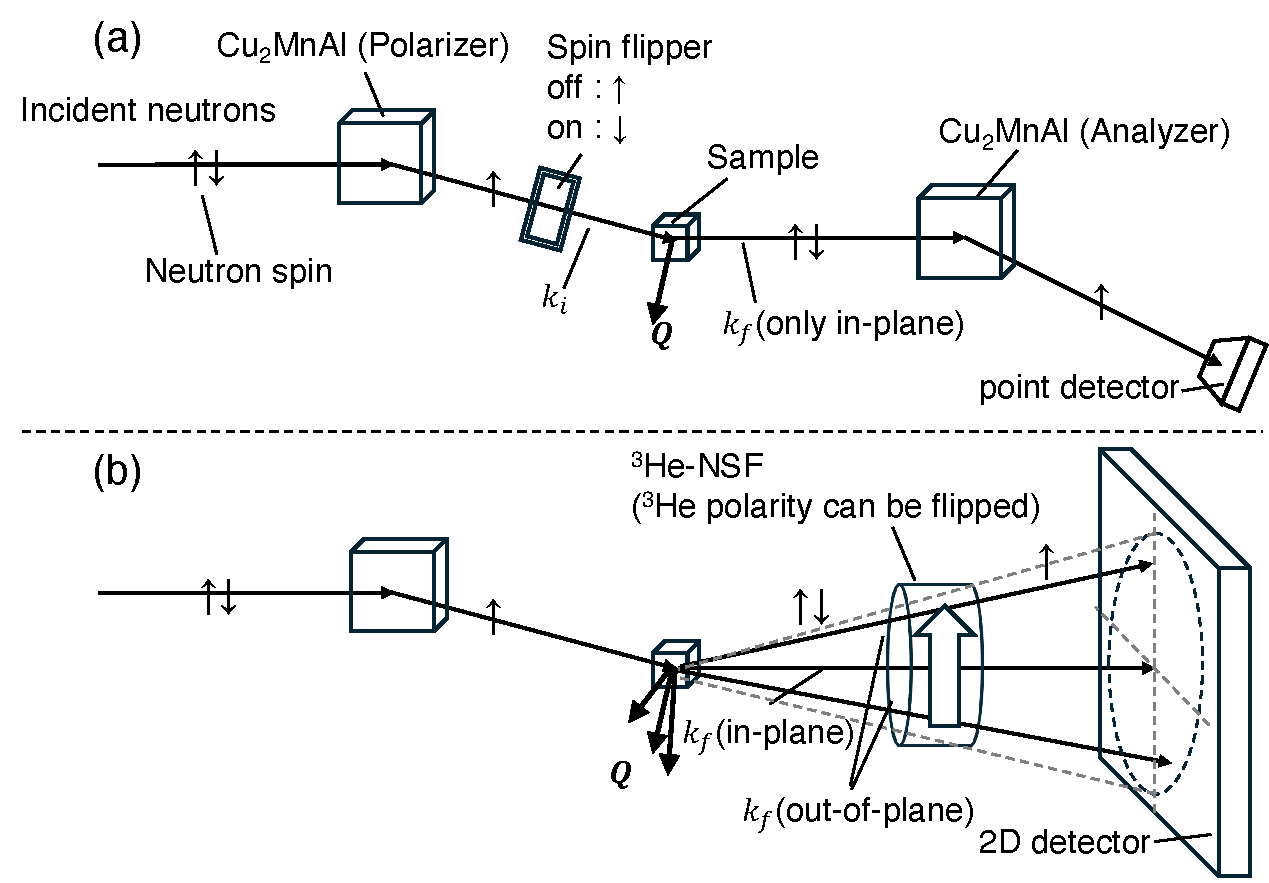
\includegraphics[width=8.5cm]{figure/Figure1_v6.pdf}
%DIFDELCMD <     %%%
\DIFdelendFL \DIFaddbeginFL 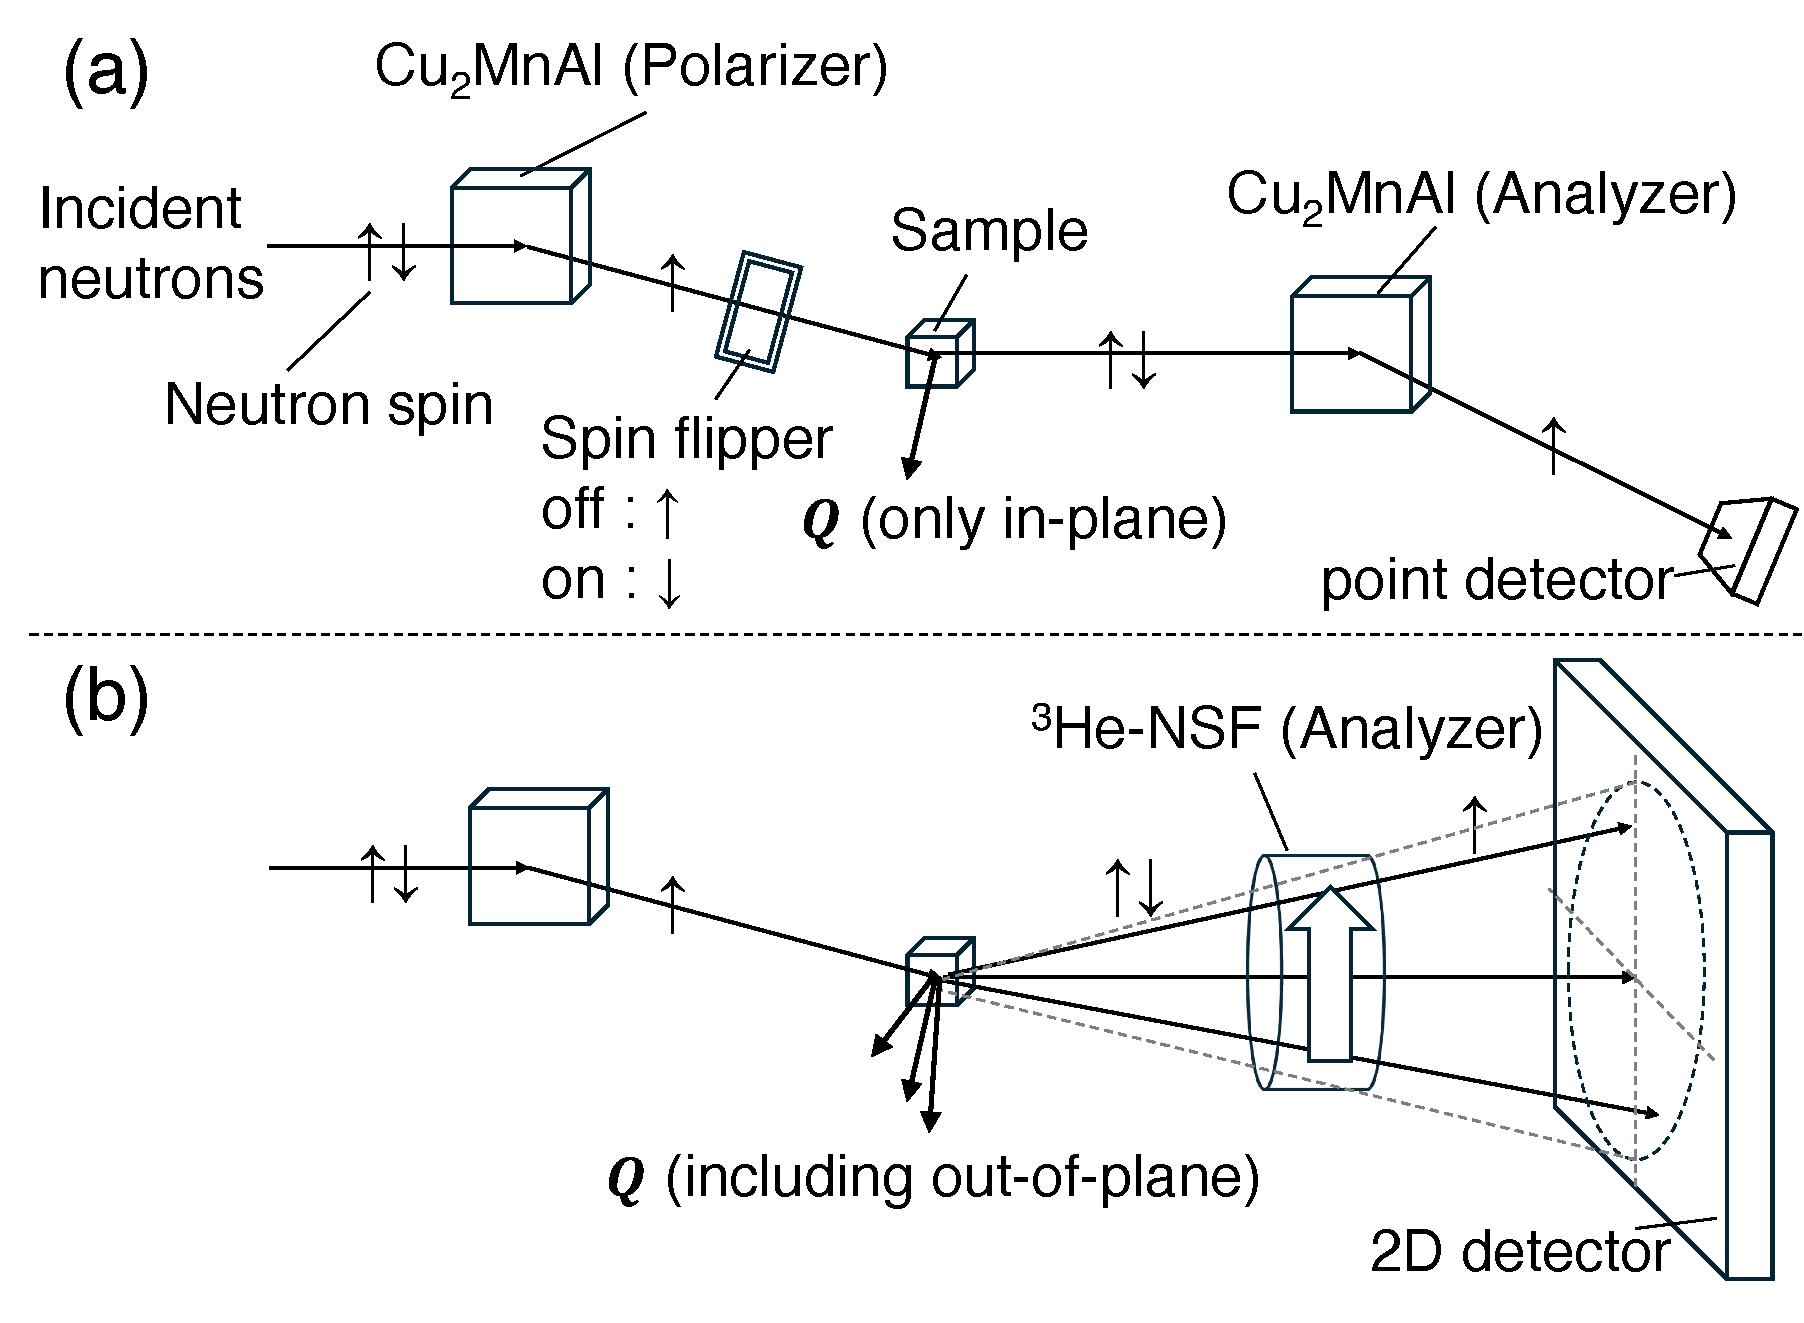
\includegraphics[width=8.5cm]{figure/Figure1_v7.pdf}
    \DIFaddendFL \caption{Schematic illustrations comparing neutron polarization analysis techniques.
(a) Conventional setup using a \ce{Cu2MnAl} crystal for both polarizer and analyzer, where only in-plane scattered neutrons are detected by a point detector.
(b) Polarization analysis setup using a \Hensf~ combined with a two-dimensional detector, enabling detection of both in-plane and out-of-plane scattered neutrons.}
    \label{fig:introduction}
\end{figure}


\section{Experimental details}


\subsection{Setup}
PONTA is one of the polarized neutron diffractometer in JRR-3, and it has a longitudinal polarization analysis option~\cite{nakajima_polarized_2024}.
In this option, both incident and scattering neutrons are polarized and analyzed by \ce{Cu2MnAl} Heusler crystal monochromator, which provides a neutron wavelength of 2.3 \AA.
In this experiment, the spin analyzer of the \ce{Cu2MnAl} Heusler crystal monochromator and point detector were not used, and \Hensf~ and two-dimensional detector were installed instead.
Figure \ref{fig:Setup} shows a \DIFdelbegin \DIFdel{detail }\DIFdelend \DIFaddbegin \DIFadd{overview }\DIFaddend of the experimental setup from the sample \DIFdelbegin \DIFdel{environment }\DIFdelend to the detector.
The neutron detector was a scintillation-type two-dimensional detector with an active area of 256 mm $\times$ 256 mm using wavelength-shifting fiber~\cite{nakamura_large-area_2012} .
The detector \DIFdelbegin \DIFdel{was located }\DIFdelend \DIFaddbegin \DIFadd{and \Hensf~ were positioned }\DIFaddend at an angle of approximately 32$^{\circ}$ relative to the incident neutron beam direction \DIFdelbegin \DIFdel{.
A sample to detector }\DIFdelend \DIFaddbegin \DIFadd{and fixed during the measurement.
The sample-to-detector }\DIFaddend distance was approximately 0.9 m.
\DIFdelbegin \DIFdel{A }\DIFdelend \DIFaddbegin \DIFadd{To maximize the solid-angle coverage, the }\DIFaddend \Hensf~ was placed as close to the sample as possible\DIFdelbegin \DIFdel{to maximize the solid-angle coverage.
The }\DIFdelend \DIFaddbegin \DIFadd{.
The vertical }\DIFaddend angular coverage of the \Hensf~ was 4.7$^{\circ}$, \DIFdelbegin \DIFdel{allowing }\DIFdelend \DIFaddbegin \DIFadd{enabling }\DIFaddend polarization analysis over approximately half of the detector area around the detector center.
To suppress the background level, a neutron guide tube covered with \ce{B4C} shielding tube was installed between the \Hensf~ and the detector.
\DIFdelbegin \DIFdel{The sample was mounted }\DIFdelend \DIFaddbegin \DIFadd{A single-crystal sample of \ce{Mn3WO6} with a volume of 8 mm$^3$ was mounted on an aluminum holder and installed }\DIFaddend in a cryostat \DIFdelbegin \DIFdel{, and the rotation angles were independently }\DIFdelend \DIFaddbegin \DIFadd{with the scattering plane set to the $(H0L)$ plane.
The rotation angles $\omega$ of the sample were }\DIFaddend adjustable to align the target reflection with the detector.
The Helmholtz coil was used to maintain the neutron spin polarization by applying a vertical magnetic field of approximately 1 mT.
The magnetic field in the \Hensf~ was oriented parallel to the beam axis, and spins of the neutrons scattered from the sample adiabatically followed the field direction \DIFdelbegin \DIFdel{.
A single-crystal sample of \ce{Mn3WO6} with a volume of 8 mm$^3$ was mounted on an aluminum holder and installed in a cryostat. The scattering plane was set to the \((H0L)\) plane.
%DIF <  \Hensf~ and two-dimensional detector were installed
%DIF <  Also, neutron guide tube was installed between \Hensf~ and two-dimensional detector to surpress the background level.
%DIF <  Here, we installed a two-dimensional neutron detector
}\DIFdelend \DIFaddbegin \DIFadd{as illustrated in Fig. \ref{fig:Setup}.
}\DIFaddend 

\begin{figure}[h]
    \centering
    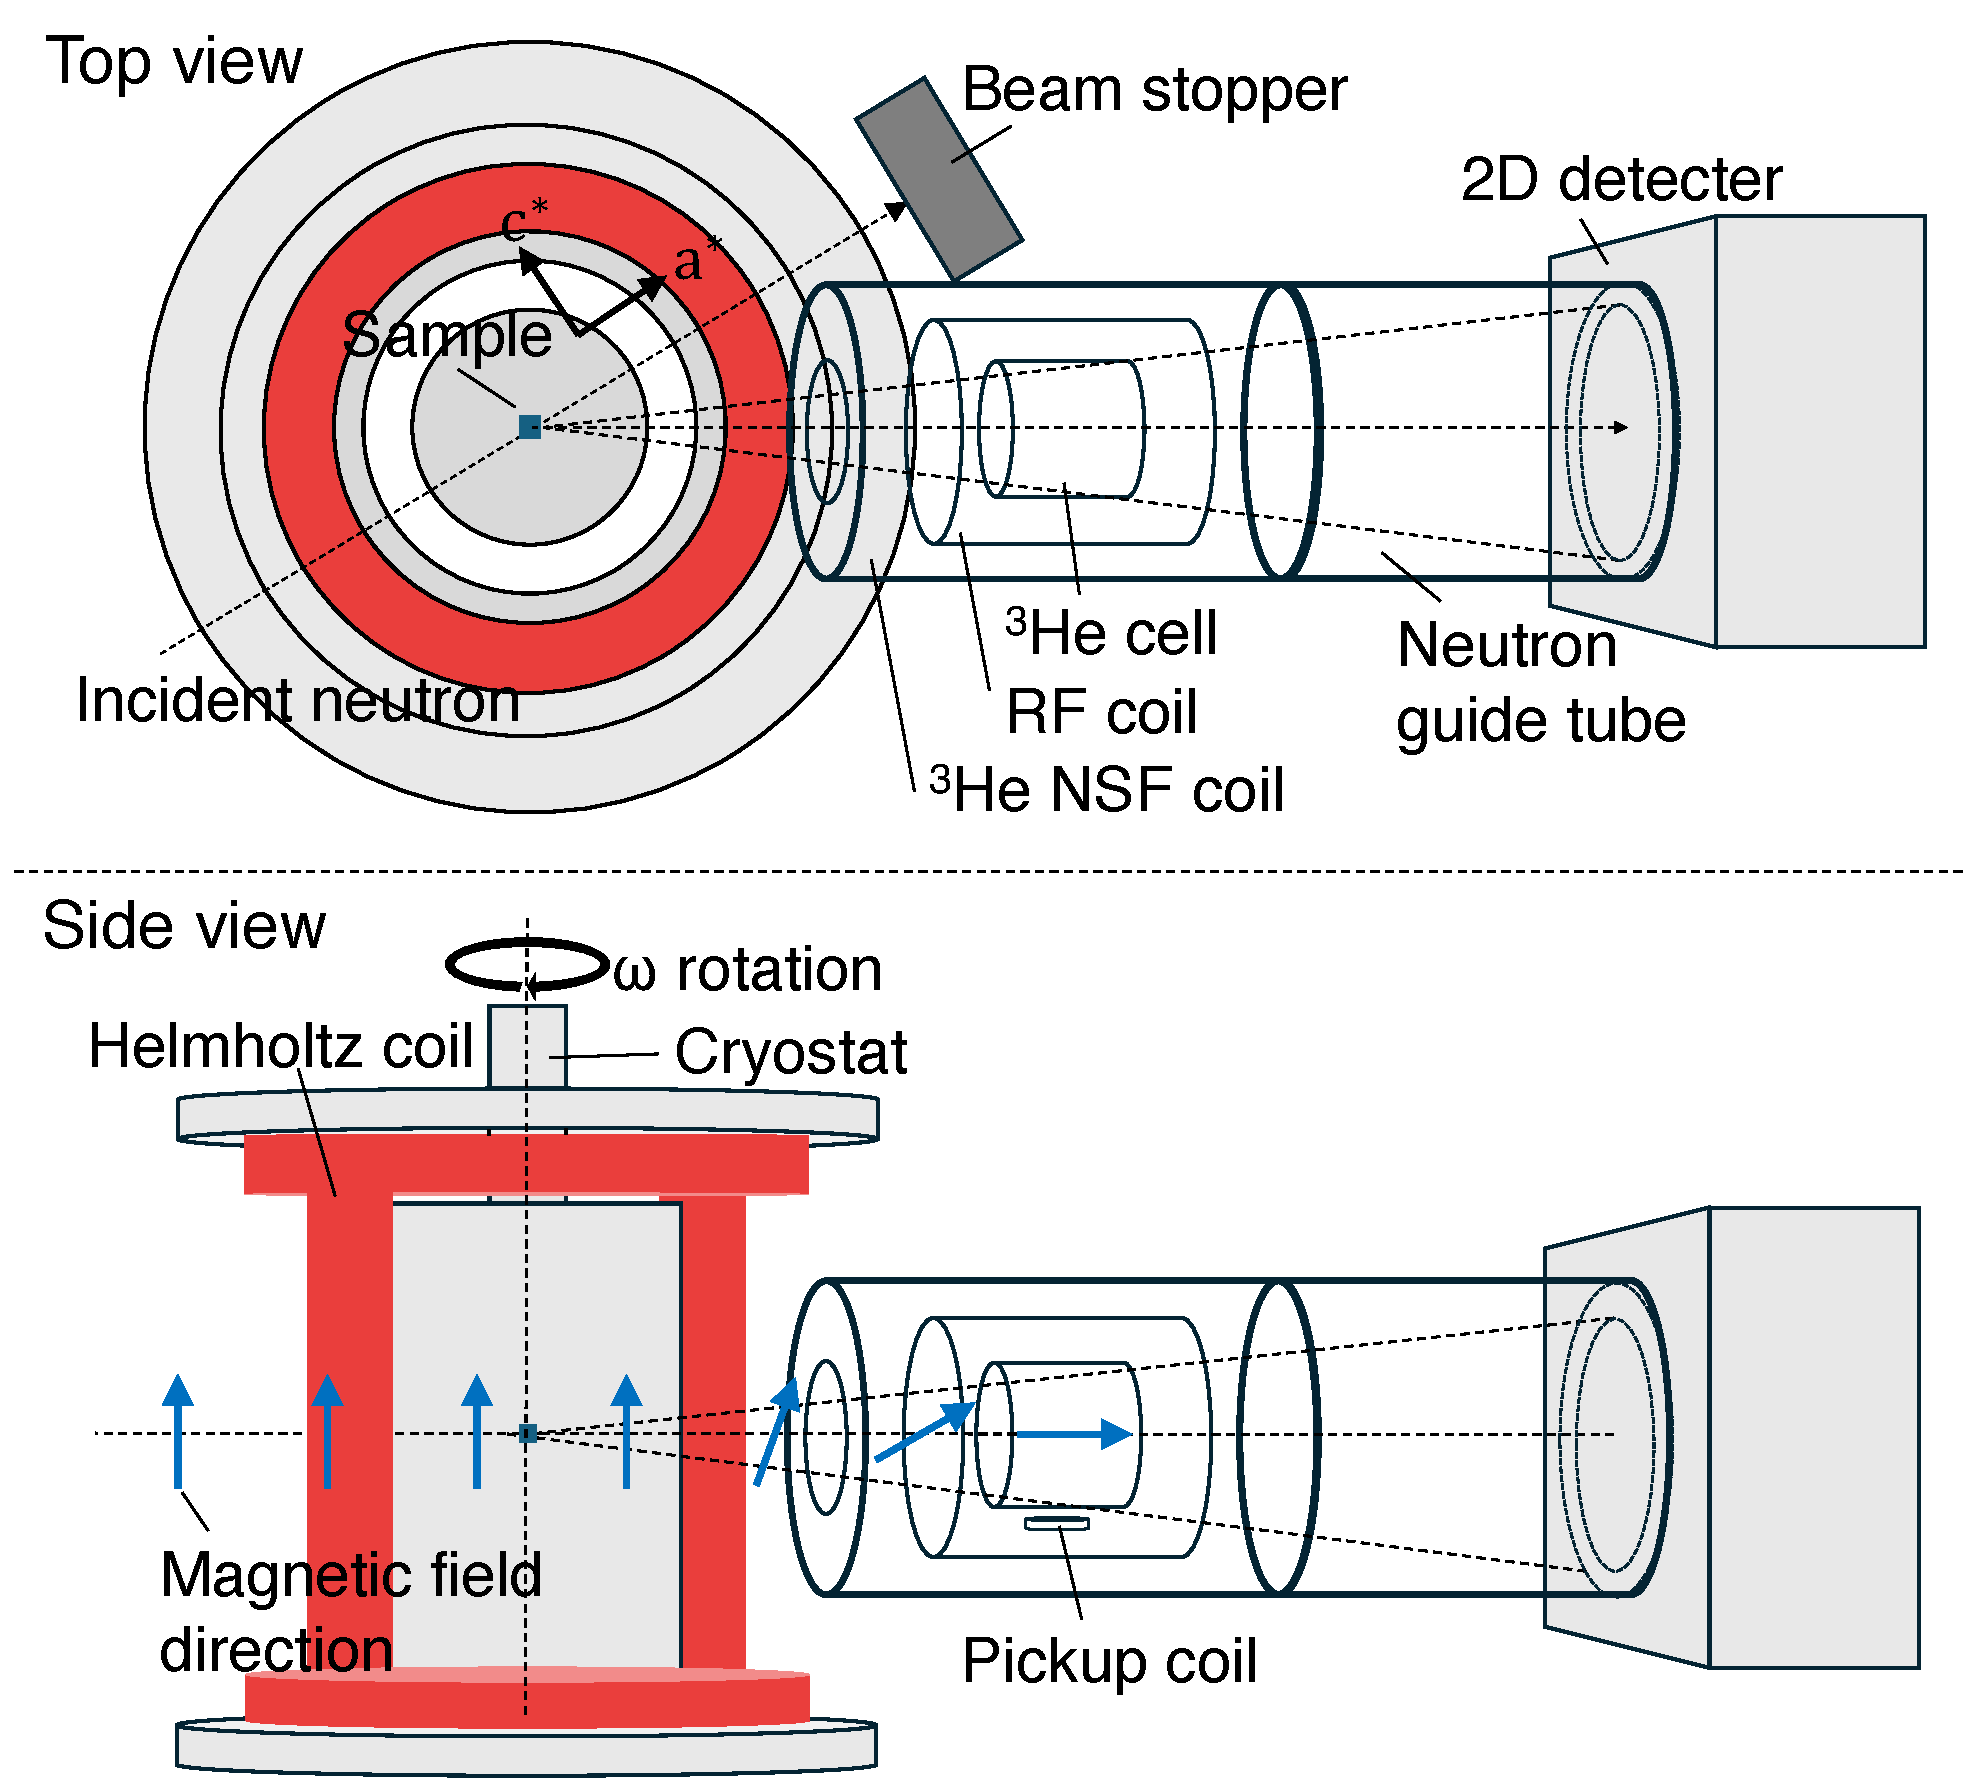
\includegraphics[width=8.5cm]{figure/Scattering_Angle_v4.pdf}
    \caption{Schematic illustration of a polarization analysis method enabling broad coverage of reciprocal lattice points in three-dimensional reciprocal space.}
    \label{fig:Setup}
\end{figure}


\subsection{\He neutron spin filter}
\begin{table*}[t]
\caption{Specifications of \He cells.}
\label{tab:He_cell}
\begin{ruledtabular}
    \begin{tabular*}{\textwidth}{lccccccc}
        Name
        & $D \times L$ (mm)
        & Volume (cm$^3$)
        & \He density (amg)
        & N$_2$ pressure (Torr)
        & K/Rb (mol)\\
        \hline
        Kenji
        & $72 \times 67$
        & 140
        & 3.2
        & 97
        & 26\\
        Shimpachi
        & $72 \times 65$
        & 146
        & 3.1
        & 100
        & 37\\
    \end{tabular*}
\end{ruledtabular}
\end{table*}
The neutron polarization principle of the \Hensf~ is based on the strong spin dependence of the neutron absorption cross section of \He nuclei.
Neutrons with spins antiparallel to the \He nuclear spins are \DIFdelbegin \DIFdel{absorbed strongly }\DIFdelend \DIFaddbegin \DIFadd{strongly absorbed}\DIFaddend , while those with spins parallel to the \He nuclear spins are transmitted.
\DIFaddbegin \DIFadd{Thus, neutron polarization requires \He gas polarization.
}\DIFaddend The \He polarization was achieved \DIFaddbegin \DIFadd{by }\DIFaddend using Spin-Exchange Optical Pumping (SEOP) method \DIFaddbegin \DIFadd{\mbox{%DIFAUXCMD
\cite{bouchiat_nuclear_1960}}\hskip0pt%DIFAUXCMD
}\DIFaddend .
In this method, circularly polarized laser light polarizes alkali-metal atoms, and the polarization is then transferred to \He nuclei through \DIFdelbegin \DIFdel{spin-exchange collisions.
An darkroom environment using the SEOP laser was constructed in the beamline experimental area.
The \He gas was polarized in the darkroom and the \He cell was transported to the beamline, where neutron measurements were performed during the relaxation of the \He polarization.
It is known as an }\textit{\DIFdel{ex-situ}} %DIFAUXCMD
\DIFdel{SEOP method.
The SEOP }\DIFdelend \DIFaddbegin \DIFadd{hyperfine interactions.
The SEOP }\DIFaddend system employed in this study was designed based on that developed for the polarized neutron spectrometer POLANO at J-PARC MLF \DIFaddbegin \DIFadd{\mbox{%DIFAUXCMD
\cite{ino_development_2017}}\hskip0pt%DIFAUXCMD
}\DIFaddend .
The SEOP system and the polarization analysis coil are equipped with a \DIFdelbegin \DIFdel{fast }\DIFdelend adiabatic fast-passage nuclear magnetic resonance (AFP NMR) system to flip the \He polarization \DIFaddbegin \DIFadd{\mbox{%DIFAUXCMD
\cite{ino_compact_2012}}\hskip0pt%DIFAUXCMD
}\DIFaddend .
An NMR pickup coil is also placed at the bottom of the \He cell to monitor the \He polarization \DIFaddbegin \DIFadd{with the NMR signal }\DIFaddend (Fig.~\ref{fig:Setup}).
Two \He glass cells\DIFaddbegin \DIFadd{, named Kenji and Shimpachi, }\DIFaddend made of aluminosilicate glass (GE180) with nearly identical dimensions were used \DIFdelbegin \DIFdel{for }\DIFdelend \DIFaddbegin \DIFadd{in }\DIFaddend the experiment.
\DIFdelbegin \DIFdel{One cell was installed on the polarized neutron experiment, while the other was being polarized in SEOP system, and the two cells were alternately exchanged during the experiment}\DIFdelend \DIFaddbegin \DIFadd{Both cells are filled with \He gas, nitrogen gas, and a mixture of alkali-metal atoms Rb and K for the hybrid SEOP \mbox{%DIFAUXCMD
\cite{babcock_hybrid_2003,chen_spin-exchange_2007}}\hskip0pt%DIFAUXCMD
}\DIFaddend .
The details of the cell specifications are described in Table \ref{tab:He_cell}.
\DIFdelbegin \DIFdel{In the table, the $D$ and $L$ represent the diameter and length }\DIFdelend \DIFaddbegin \DIFadd{An darkroom for using the SEOP laser was constructed in the beamline experimental area.
The \He gas was polarized in the darkroom.
After the saturation, the \He cell was transported to the beamline, where neutron measurements were performed during the relaxation }\DIFaddend of the \He \DIFdelbegin \DIFdel{glass cell , respectively}\DIFdelend \DIFaddbegin \DIFadd{polarization.
It is known as an }\textit{\DIFadd{ex-situ}} \DIFadd{\Hensf~ method.
Because the \He polarization decreases with time in this method, one cell was used for the polarized neutron experiment while the other was polarized in the SEOP system, and the two cells were alternately exchanged every two or three days during the experiment}\DIFaddend .

\section{Results}
In this section, \DIFaddbegin \DIFadd{we present }\DIFaddend the results of polarized neutron diffraction experiments on \ce{Mn3WO6} \DIFdelbegin \DIFdel{are presented.
First, nuclear Bragg reflections of \ce{Mn3WO6} were used to evaluate the performance of the \Hensf and to determine the \He polarization and relaxation timerequired for polarization correction.
Then, }\DIFdelend \DIFaddbegin \DIFadd{performed to demonstrate polarization analysis using a \Hensf~ combined with a two-dimensional detector.
Figure~\ref{fig:procedure} shows the procedures for data acquisition and data reduction of }\DIFaddend polarization-analysis \DIFdelbegin \DIFdel{results for magnetic reflections of \ce{Mn3WO6} extracted from }\DIFdelend \DIFaddbegin \DIFadd{results for magnetic reflections distributed in }\DIFaddend three-dimensional \DIFaddbegin \DIFadd{reciprocal space.
The data were acquired by scanning the sample rotation angle $\omega$.
For each measurement, the \He polarization was flipped by AFP NMR to switch the analyzer condition between $I^{++}$ and $I^{+-}$.
Because an }\textit{\DIFadd{ex-situ}} \DIFadd{\Hensf~was employed, \He polarization was gradually decayed during the experiment, the neutron polarization and transmission of the \Hensf~ also decreased with time.
Therefore, corrections for these time-dependence are nesessary.
For this correction, the time dependence of the \He polarization was evaluated from the nuclear Bragg reflection.
After applying these time-dependence correction, the detector coordinates and sample rotation angle were transformed into }\DIFaddend reciprocal-space \DIFdelbegin \DIFdel{data are described}\DIFdelend \DIFaddbegin \DIFadd{coordinates}\DIFaddend .

\DIFdelbegin %DIFDELCMD < \begin{figure}[h]
%DIFDELCMD <     %%%
\DIFdelendFL \DIFaddbeginFL \begin{figure}[t]
    \DIFaddendFL \centering
    \DIFdelbeginFL %DIFDELCMD < 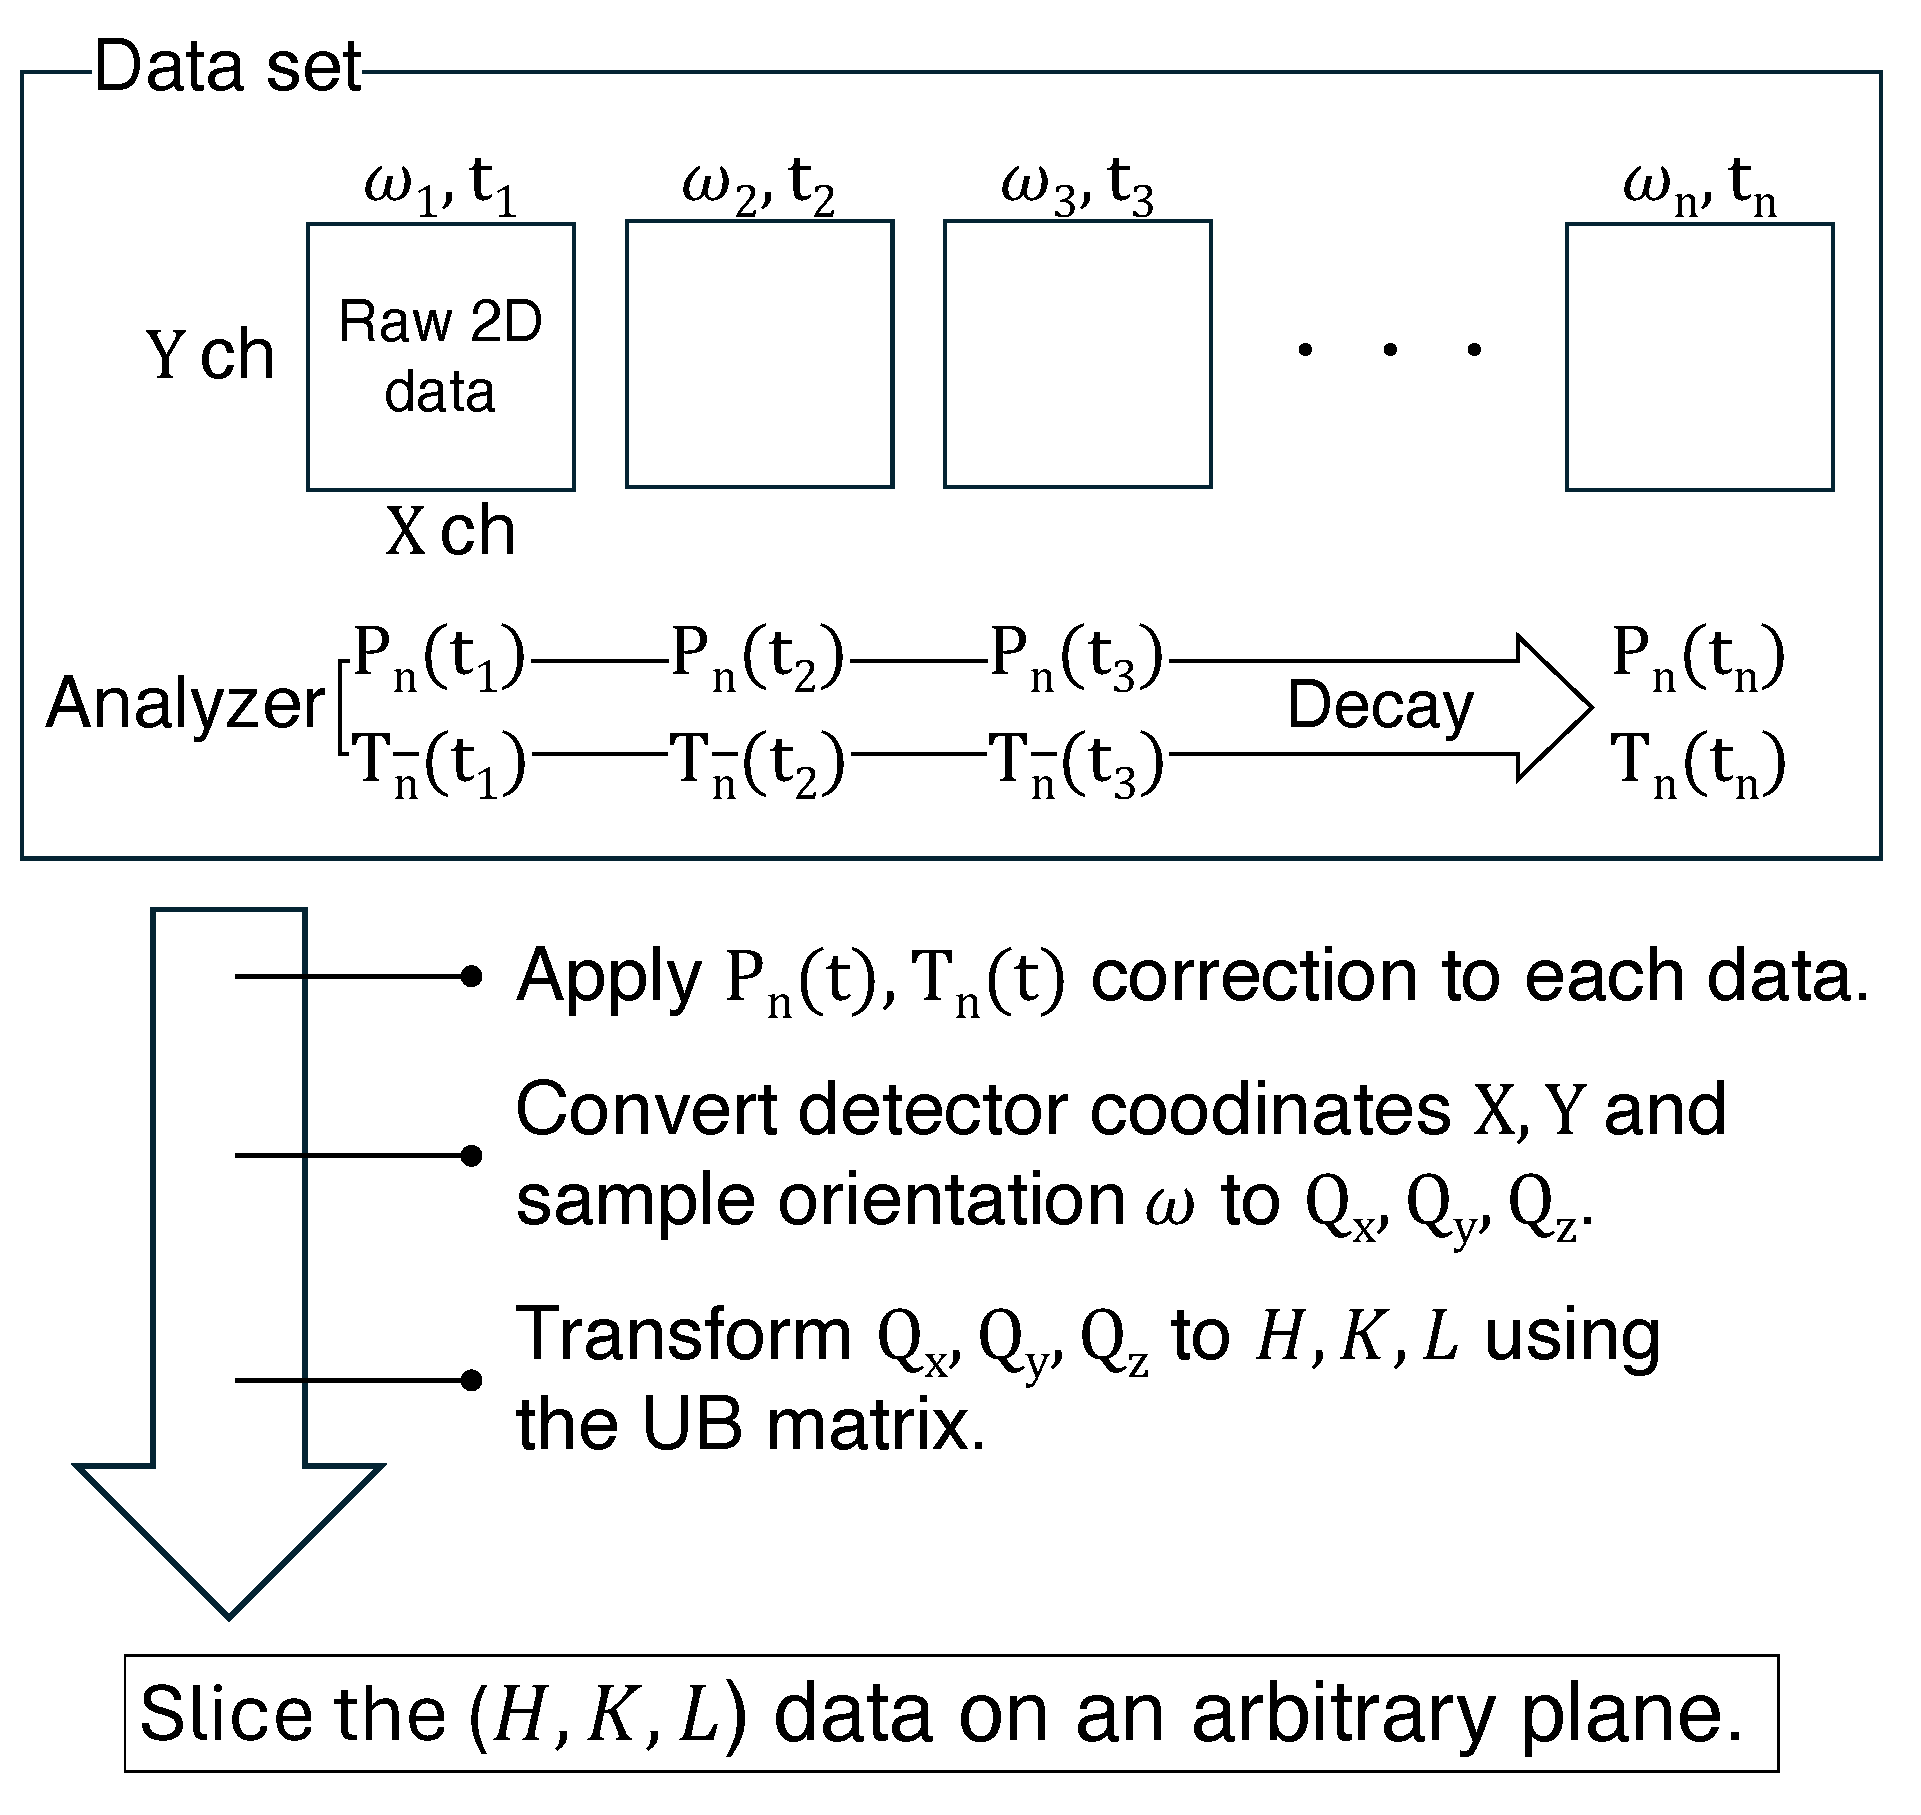
\includegraphics[width=8.5cm]{figure/Procedure_v1.pdf}
%DIFDELCMD <     %%%
\DIFdelendFL \DIFaddbeginFL 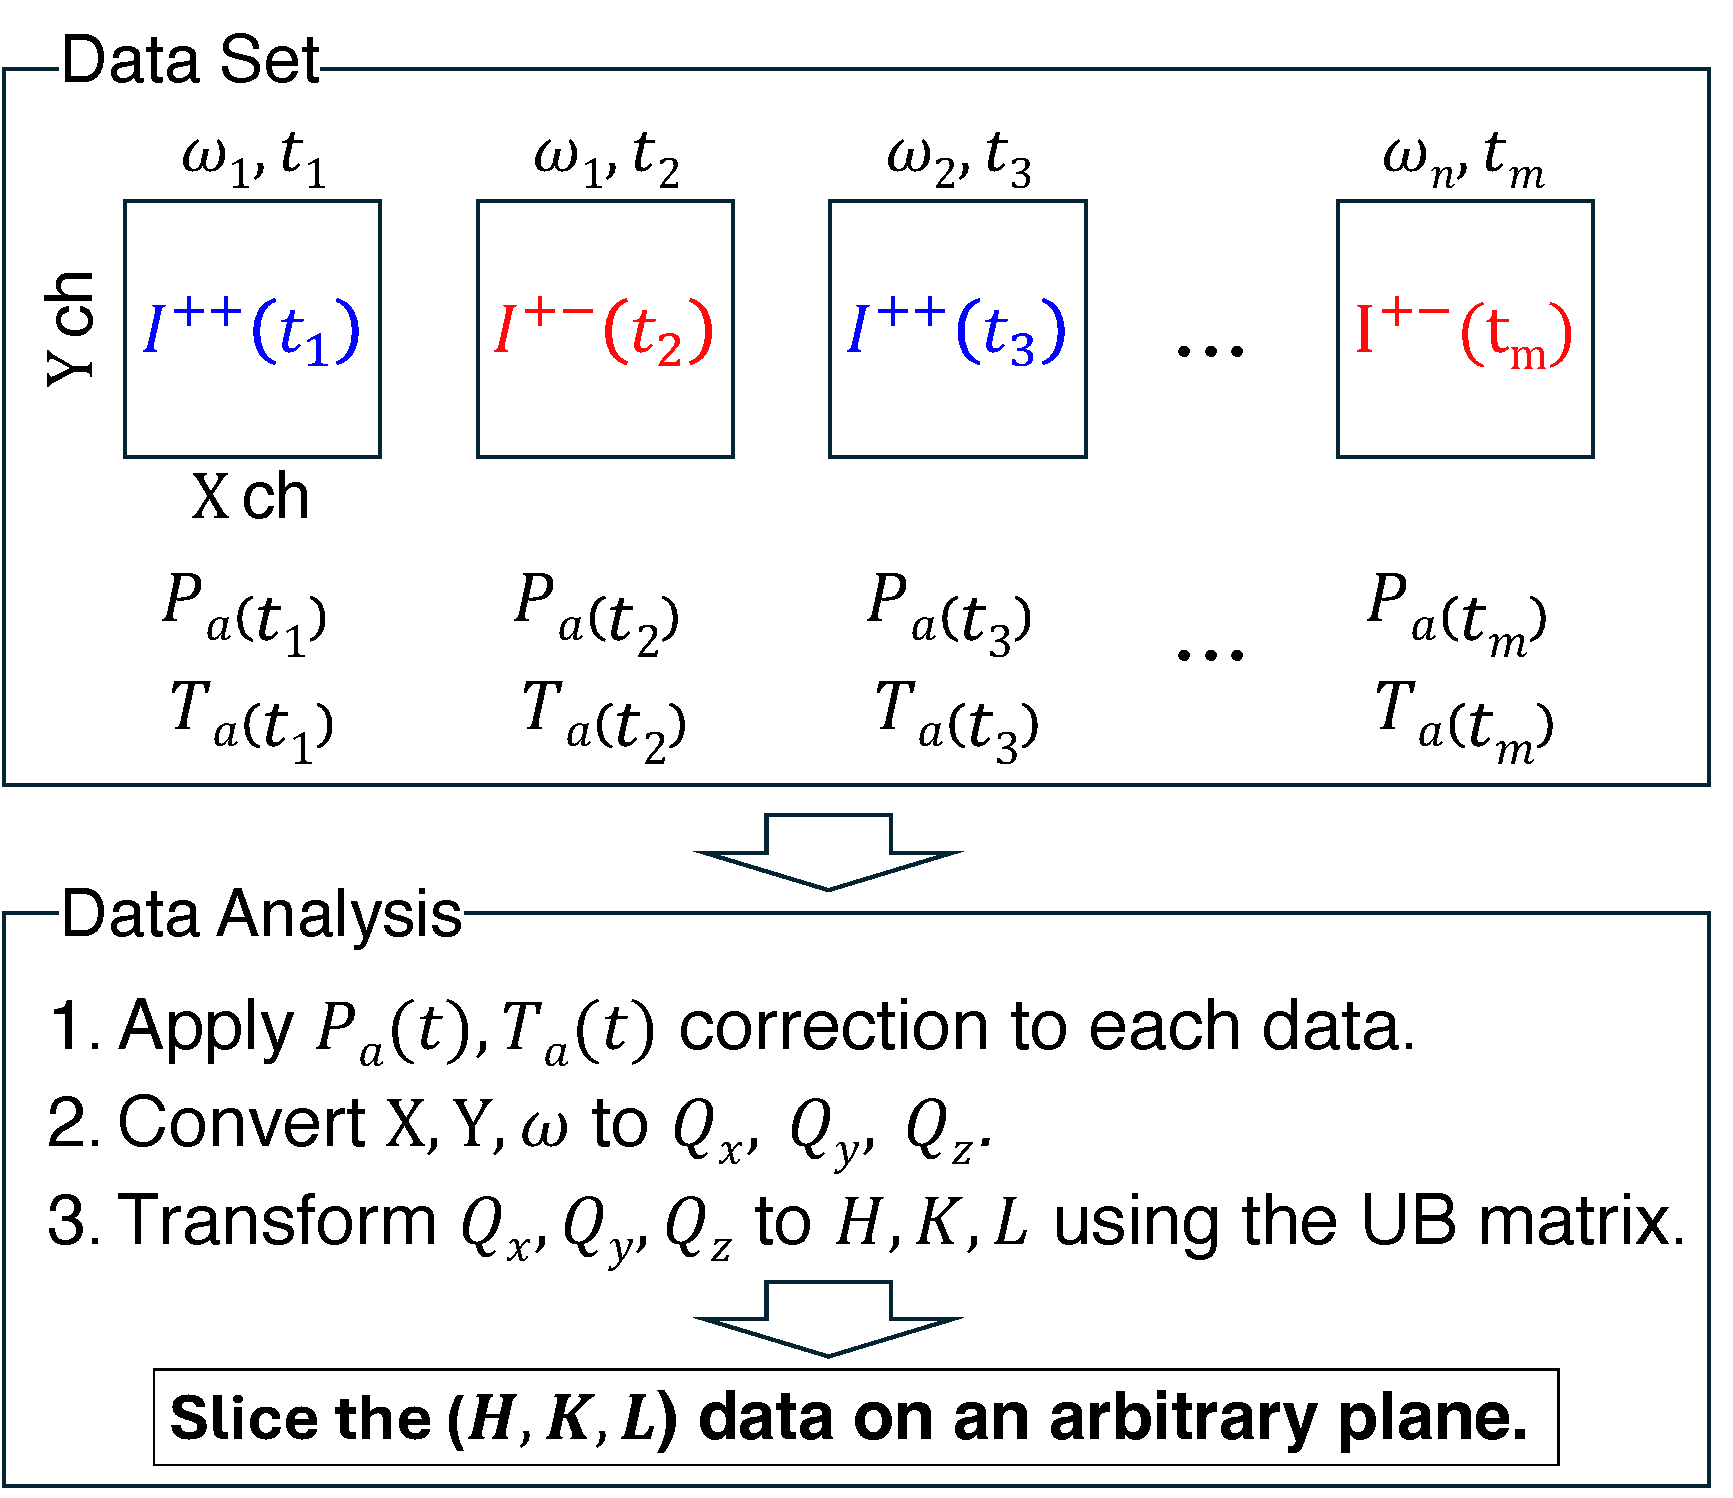
\includegraphics[width=\columnwidth]{figure/Procedure_v2.pdf}
    \DIFaddendFL \caption{
    Schematic diagram of the data-reduction procedure for polarization analysis using an \textit{ex-situ} \Hensf and a two-dimensional detector.
    Raw two-dimensional detector data measured at different sample rotation angles $\omega_i$ and times $t_i$ are corrected using the time-dependent neutron polarization $P_n(t_i)$ and transmission $T_n(t_i)$.
    The detector coordinates (X,Y) and sample rotation angle $\omega$ are converted to $Q_x,Q_y,Q_z,$ and then transformed to $H,K,L$ using the UB matrix.
    The corrected three-dimensional reciprocal-space data can then be sliced on an arbitrary plane.
    }
    \label{fig:procedure}
\end{figure}



\subsection{\DIFdelbegin \DIFdel{Performance }\DIFdelend \DIFaddbegin \DIFadd{Evaluation }\DIFaddend of \He neutron spin filter \DIFaddbegin \DIFadd{from nuclear scattering}\DIFaddend }
\DIFaddbegin \label{sec:He-3}
\begin{figure}[t]
    \centering
    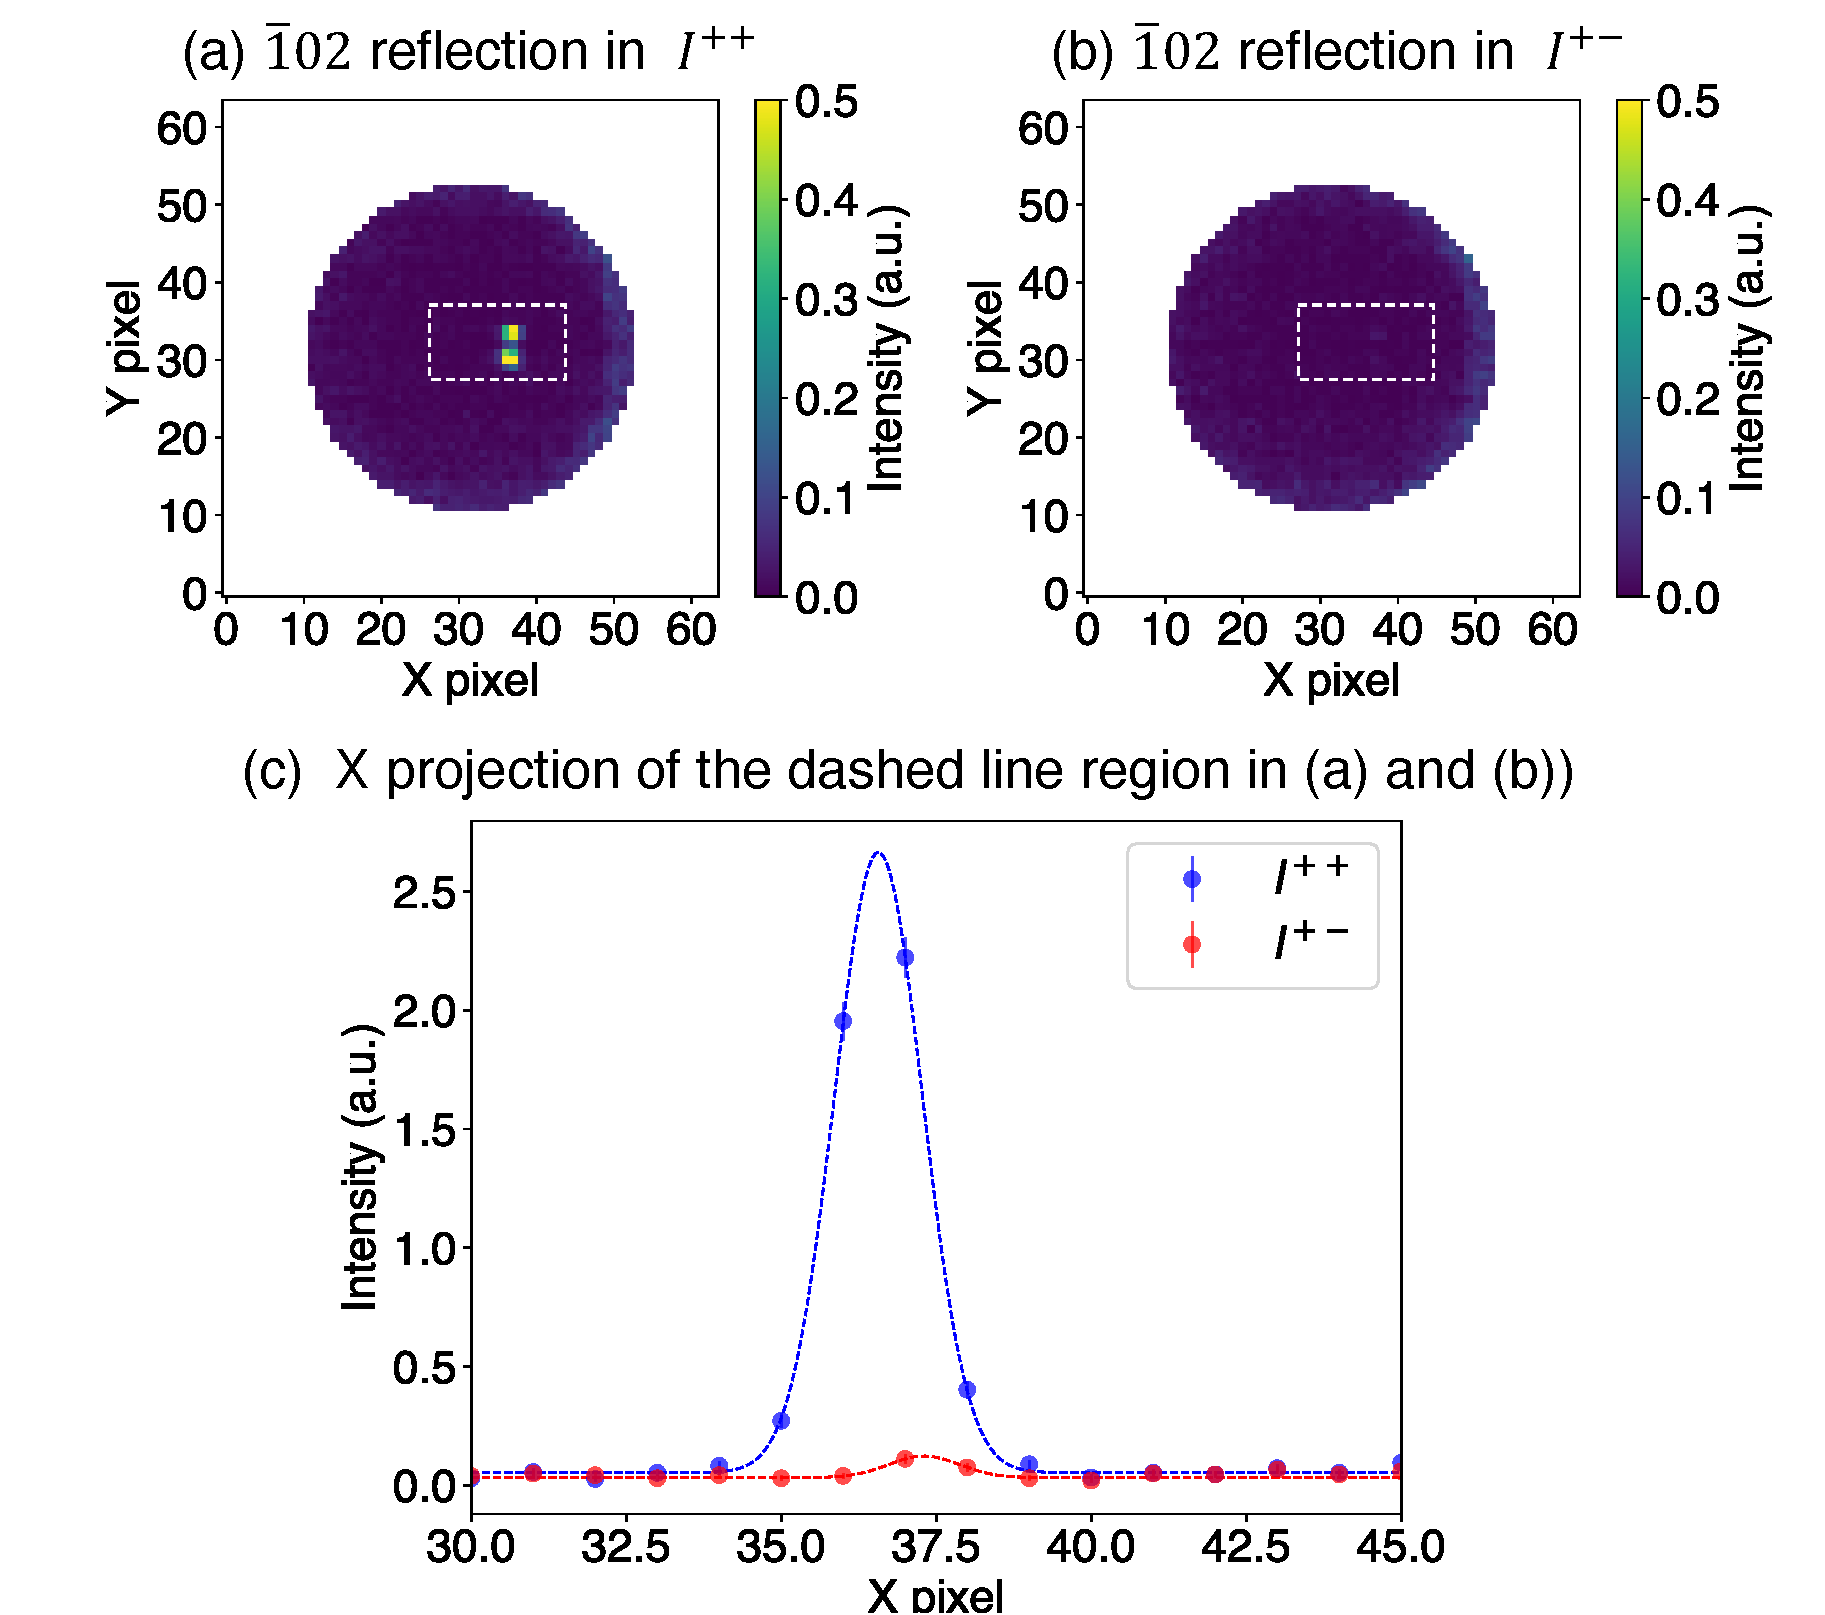
\includegraphics[width=\columnwidth]{figure/raw_data_v8.pdf}
    \caption{
    \DIFaddFL{(a) Non-spin-flip intensity ($I^{++}$) and (b) spin-flip intensity ($I^{+-}$) maps, showing only the region covered by the \He cell.
    A clear difference in the intensity of the $\bar{1}02$ nuclear Bragg peak is observed depending on the direction of the \He polarization.
    (c) Line profile along the (x) direction obtained by integrating the intensity within the dashed regions in (a) and (b).
    }}
    \label{fig:rawdata}
\end{figure}
\DIFaddend The \He polarization was estimated from the nuclear Bragg peak intensity of \ce{Mn3WO6} single crystal sample.
Nuclear peak intensities where the incident neutrons polarized by \ce{Cu2MnAl} single crystal monochromator and scattering neutrons analyzed by \Hensf~ were given by the following equations:
\begin{align}
    I^{+\pm}(t) &= N_0 \Sigma^{++}T_pT_a(t)(1\pm P_pP_a(t))
    \label{eq:int_bragg}
\end{align}
where the supersucripts of $I^{+\pm}$ indicate the incident neutron polarization state and the scattered neutron polarization state, respectively,
$N_0$ is a number of incident neutrons comes from the reactor source, $\Sigma^{++}$ represents the scattering cross section of the \DIFdelbegin \DIFdel{($10\bar{2}$) }\DIFdelend \DIFaddbegin \DIFadd{$\bar{1}02$ }\DIFaddend nuclear reflection of \ce{Mn3WO6},
$T_p$ is the neutron transmission of the \ce{Cu2MnAl} \DIFdelbegin \DIFdel{monochromator}\DIFdelend \DIFaddbegin \DIFadd{polarizer}\DIFaddend , $T_a(t)$ is the neutron transmission of the \Hensf\DIFdelbegin \DIFdel{~ at time $t$}\DIFdelend ,
$P_p$ is the neutron polarization of the \ce{Cu2MnAl} \DIFdelbegin \DIFdel{monochromator}\DIFdelend \DIFaddbegin \DIFadd{polarizer}\DIFaddend , and $P_a(t)$ is the neutron polarization of the \Hensf.
%DIF <  式\ref{eq:int_bragg}において、$I^{++}$と$I^{+-}$を足し合わせることで以下の式が得られる。
By summing $I^{++}$ and $I^{+-}$ in Eq~\ref{eq:int_bragg}, the following expression is obtained:
\begin{align}
    I^{++}(t)+I^{+-}(t) = 2N_0 \Sigma^{++}T_pT_a(t),
    \label{eq:transmission}
\end{align}
Here, the measurement time is sufficiently short compared with the relaxation time of the polarized \He gas, $I^{++}(t)$ and $I^{+-}(t)$ can be regarded as being measured at the same time.
%DIF <  ここで、$t$は偏極した\He の緩和時間と比較して短時間の測定であるため、$I^{++}(t)$と$I^{+-}(t)$は同一の時間に測定されているとみなしている。
%DIF <  \Hensfの中性子透過率$T_a(t)$と\He 偏極度$P_\mathrm{He}(t)$は、以下の式で表される。
The neutron transmission $T_a(t)$ of \Hensf, the neutron polarization $P_a(t)$ of \Hensf, and \He polarization $P_\mathrm{He}(t)$ are given by the following equations \DIFaddbegin \DIFadd{\mbox{%DIFAUXCMD
\cite{coulter_neutron_1990}}\hskip0pt%DIFAUXCMD
}\DIFaddend ,
\begin{align}
    T_a(t) &= T_\mathrm{cell}\exp(-\rho d \sigma(\lambda))\cosh(\rho d \sigma(\lambda)P_\mathrm{He}(t)),\\
    P_a(t) &= \tanh(\rho d \sigma(\lambda)P_\mathrm{He}(t)),\\
    P_\mathrm{He}(t) &= P_0 \exp(-t/\tau),
    \label{eq:transmission_3He}
\end{align}
where $T_\mathrm{cell}$ is the transmission of the \He glass cell, $\rho$ is a number density of \He, $d$ is a gas thickness of \He,
$\sigma (\lambda)$ is a neutron absorption cross section of unpolarized \He,
$P_0$ is the initial polarization at $t=0$, and $\tau$ is the relaxation time.
The wavelength $\lambda$ of the incident neutrons was monochromatized to 2.36 \AA~by \ce{Cu2MnAl}.
%DIF <  ここでPONTAでは、入射中性子の波長$\lambda$は2.36 \AAに単色化されている。
%DIF <  そのため\He 偏極度が0 ($P_\mathrm{He} = 0$)のときの強度$I_\mathrm{unpol}$との比をとることで、以下の式が得られる。
By taking the ratio with the intensity $I_\mathrm{unpol}$ measured when the \He polarization is zero ($P_\mathrm{He} = 0$), the following equation is obtained,
\begin{align}
    \frac{I^{++}(t)+I^{+-}(t)}{I_\mathrm{unpol}} = 2\cosh(\rho d \sigma(\lambda)P_\mathrm{He}(t)).
    \label{eq:transmission_ratio}
\end{align}
The \He gas thickness $\rho d$ was determined from the transmission ratio between the \He cell and an empty cell of the same size\DIFdelbegin \DIFdel{and was then used to evaluate \He polarization $P_\mathrm{He}(t)$.
%DIF <  \He ガス厚さ$\rho d$については\He が封入されていない同サイズの空セルとの比を取ることで求め、\He 偏極度$P_\mathrm{He}(t)$を求めた。
%DIF <  By adding these two intensities and taking their ratio to the intensity measured with unpolarized \He ($P_\mathrm{He}=0$), the following equation is obtained:
%DIF <  \begin{equation}
%DIF <      \frac{I^{++}+I^{+-}}{I_\mathrm{unpol}} = 2\cosh(\rho d \sigma(\lambda) P_\mathrm{He}).
%DIF <      \label{eq:int_bragg_ratio}
%DIF <  \end{equation}
%DIF <  The product $\rho d$ was determined from the intensity ratio of the (102) nuclear Bragg peak measured with the unpolarized $^3$He-filled cell  to that measured with the empty cell.
}\DIFdelend \DIFaddbegin \DIFadd{.
The value of $\rho d$ was $18.5 \pm 0.5\ [\textrm{amg cm}]$ for Kenji cell and $18.8 \pm 0.4\ [\textrm{amg cm}]$ for Shimpachi cell.
Note that the amagat is a non-SI unit of the volumetric number density of an ideal gas at 0 $^{\circ}$C (273.15 K) and 1 atm (101.325 kPa), and one amagat is equivalent to $2.69\times 10^{19} /\textrm{cm}^3$.
}\DIFaddend 

Figure \ref{fig:rawdata} (a,b) shows two-dimensional intensity maps measured just after transporting the \DIFdelbegin \DIFdel{\He cell ($P_\mathrm{He}(t=0)$}\DIFdelend \DIFaddbegin \DIFadd{Shimpachi cell ($P_\mathrm{He}(0)$}\DIFaddend ), where the \DIFdelbegin \DIFdel{($10\bar{2}$) nuclear Bragg peak }\DIFdelend \DIFaddbegin \DIFadd{$\bar{1}02$ nuclear reflection }\DIFaddend intensity clearly changes depending on the \DIFdelbegin \DIFdel{\He polarity between up (}\DIFdelend $I^{++}$ \DIFdelbegin \DIFdel{) and down (}\DIFdelend \DIFaddbegin \DIFadd{and }\DIFaddend $I^{+-}$\DIFdelbegin \DIFdel{).
%DIF <  これらの強度マップからピーク領域を切り出してx軸方向に投影したものが右のグラフである。
}\DIFdelend \DIFaddbegin \DIFadd{.
}\DIFaddend Figure \ref{fig:rawdata} (c) shows the result of projecting the peak region of these intensity maps along the x-axis.
\DIFdelbegin \DIFdel{By integrating the peak intensity and using Eq.\ref{eq:transmission_ratio}, the \He polarization was determined to be $P_\mathrm{He} = 0.81 \pm 0.05$.%DIF <  ピーク強度を積分して式\ref{eq:transmission_ratio}から\He 偏極度を求めた結果、$P_\mathrm{He} = 0.81 \pm 0.05$であった。
Throughout the experiment, nuclear scattering measurements were periodically conducted between magnetic scattering measurements}\DIFdelend \DIFaddbegin \DIFadd{The peak intensities for $I^{++}$ and $I^{+-}$ were integrated, and $I_\mathrm{unpol}$ was also integrated in the same region before polarizing \He by SEOP.
The \He polarization was then determined using Eq.~\ref{eq:transmission_ratio}, yielding $P_\mathrm{He} = 0.81 \pm 0.05$ for the Shimpachi cell}\DIFaddend .
Figure~\ref{fig:pol_trans_decay} shows the time evolution of the \He polarization determined from the nuclear reflection (open circles) and the NMR signal (closed circles).
\DIFdelbegin \DIFdel{The }\DIFdelend \DIFaddbegin \DIFadd{Throughout the experiment, nuclear scattering measurements were periodically conducted between magnetic scattering measurements.
The time evolution of the nuclear reflection intensities and the NMR signal showed good agreement and the }\DIFaddend relaxation time $\tau$ was estimated to be \DIFdelbegin \DIFdel{$\tau = 130.9 \pm 0.5$ }\DIFdelend \DIFaddbegin \DIFadd{$\tau = 131.1 \pm 0.7$ }\DIFaddend hour.
Figure~\ref{fig:pol_trans_decay} also shows the neutron polarization and transmission calculated \DIFdelbegin \DIFdel{using these values.
The cellwas replaced approximately every two days during the experiment}\DIFdelend \DIFaddbegin \DIFadd{from eq.~\ref{eq:transmission_3He} using Shimpachi cell.
Also, the same measurement and analysis were performed for the Kenji cell,yielding $P_\mathrm{He}(0) = 0.72 \pm 0.06$ and $\tau = 128.0 \pm 0.3$ hour.
$P_p$ is also required for the polarization correction of the magnetic scattering data.
The asymmetry between $I^{++}$ and $I^{+-}$ is described by Eq.~\ref{eq:int_bragg},
}\begin{equation}
\DIFadd{\frac{I^{++}-I^{+-}}{I^{++}+I^{+-}} = P_pP_a(t).
}\end{equation}
\DIFadd{Since $P_a(t)$ is independently determined from the \He polarization, $P_p$ can be obtained and the average value of $P_p$ was found to be $0.86 \pm 0.06$.
Note that $P_p$ was determined for each nuclear reflection measurement and includes the effects of environmental background variations and neutron depolarization in the guide field in the analysis}\DIFaddend .
The validity of the polarization correction was confirmed using the \DIFdelbegin \DIFdel{nuclear }\DIFdelend \DIFaddbegin \DIFadd{$\omega$ scan of $\bar{1}02$ }\DIFaddend reflection.
The \DIFaddbegin \DIFadd{integrated intensity at each $\omega$ was obtained by integrating the intensity within the peak region identified on the two-dimensional detector in Fig.~\ref{fig:rawdata}.
The }\DIFaddend raw intensity profiles of the \DIFdelbegin \DIFdel{nuclear }\DIFdelend \DIFaddbegin \DIFadd{$\bar{1}02$ }\DIFaddend reflection show a finite spin-flip intensity owing to the imperfect neutron polarization, as shown in Fig.~\ref{fig:polcorrection}(a).
By applying the polarization correction\DIFdelbegin \DIFdel{using the obtained \He polarization, the time-dependent changes in the }\DIFdelend \DIFaddbegin \DIFadd{, the }\DIFaddend neutron polarization and transmission \DIFdelbegin \DIFdel{of the \Hensf~ were corrected , }\DIFdelend \DIFaddbegin \DIFadd{were corrected and the non-spin flip and spin-flip scattering cross-sections, $\Sigma^{++}$ and $\Sigma^{+-}$, are obtained }\DIFaddend as shown in Fig.~\ref{fig:polcorrection}(b).
\DIFdelbegin \DIFdel{These values were used for the polarization correction of the magnetic scattering data}\DIFdelend \DIFaddbegin \DIFadd{Since only the non-spin-flip scattering cross section $\Sigma^{++}$ is expected for nuclear scattering, the result indicates that the polarization correction was successfully performed}\DIFaddend .
Details of the polarization correction are described in the Appendix \ref{appendix}.
\DIFaddbegin \DIFadd{These values were used for the polarization correction of the magnetic scattering data.
}\DIFaddend 

\begin{figure}[h]
    \centering
    \DIFdelbeginFL %DIFDELCMD < 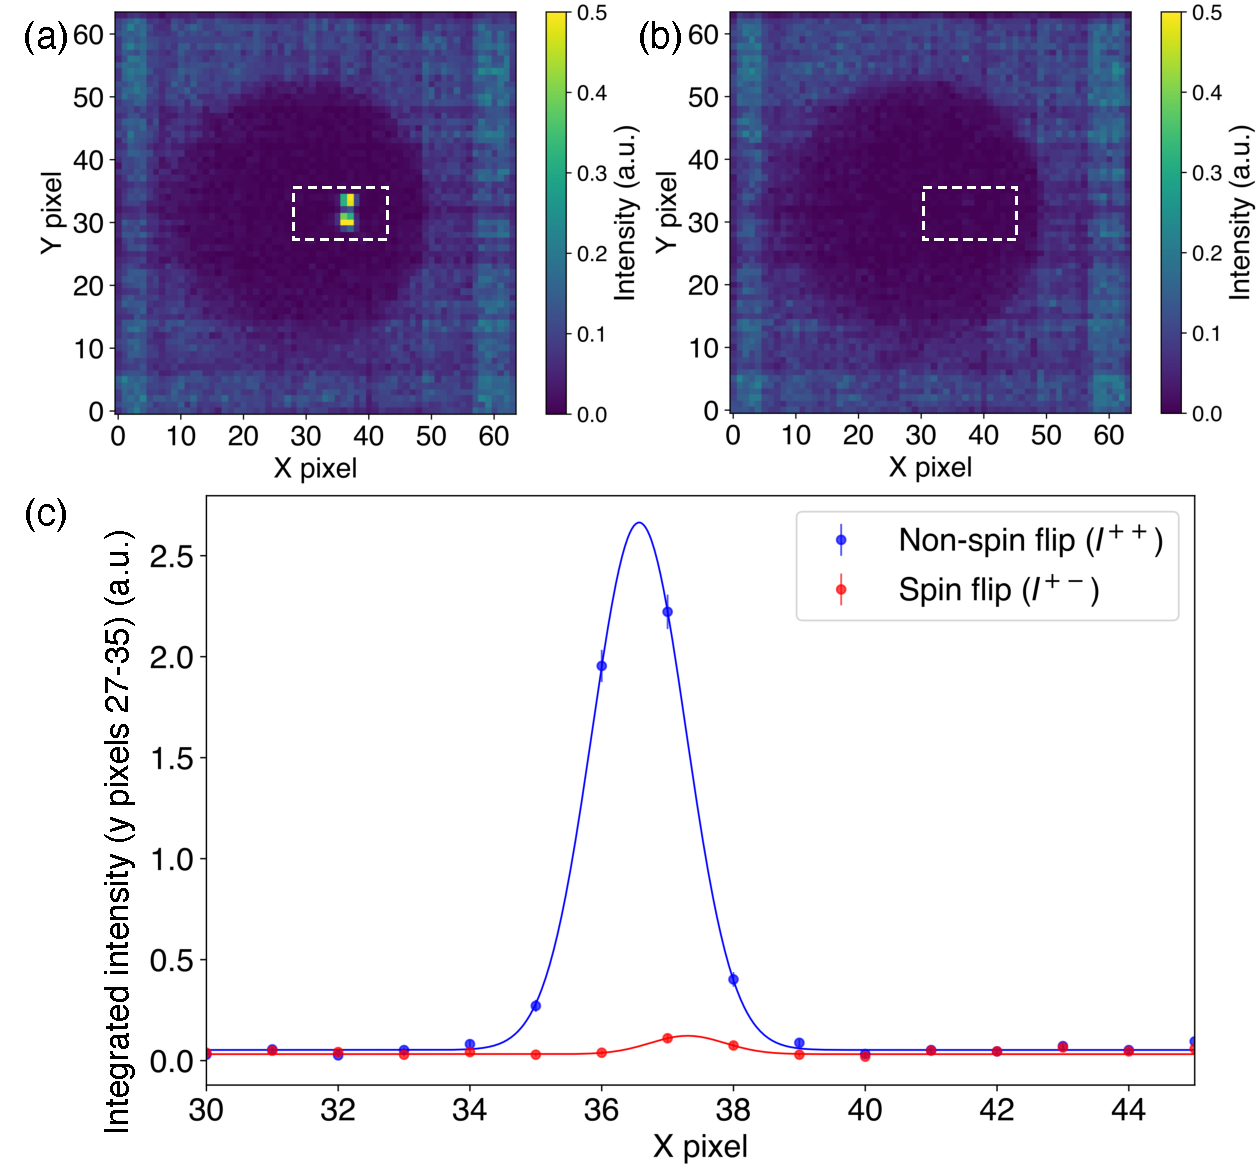
\includegraphics[width=8.5cm]{figure/raw_data_v7.pdf}
%DIFDELCMD <     %%%
\DIFdelendFL \DIFaddbeginFL 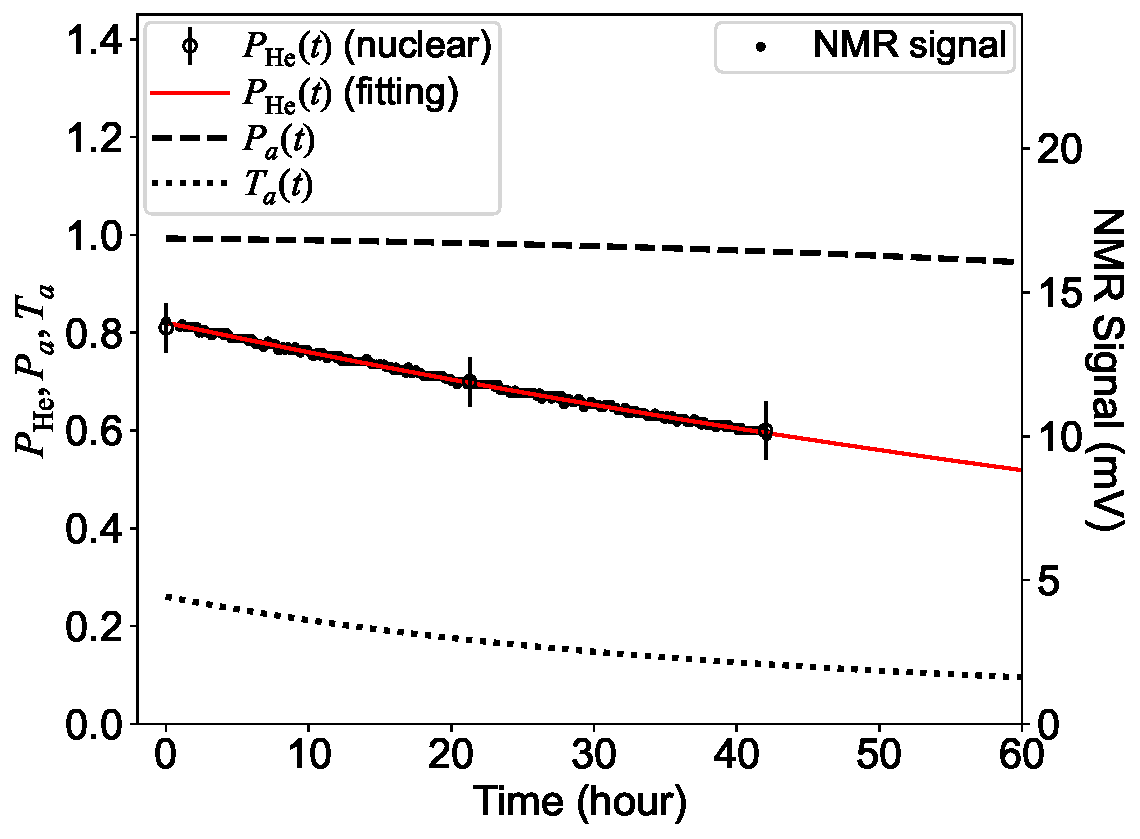
\includegraphics[width=\columnwidth]{figure/NMR_vs_time_20260530.pdf}
    \DIFaddendFL \caption{\DIFdelbeginFL \DIFdelFL{(a) Non-spin-flip ($I^{++}$) }\DIFdelendFL 
    \DIFaddbeginFL \DIFaddFL{Time dependence of the \He polarization, neutron polarization, }\DIFaddendFL and \DIFdelbeginFL \DIFdelFL{(b) spin-flip ($I^{+-}$) scattering intensity maps}\DIFdelendFL \DIFaddbeginFL \DIFaddFL{neutron transmission}\DIFaddendFL .
    \DIFdelbeginFL \DIFdelFL{A clear difference in }\DIFdelendFL \DIFaddbeginFL \DIFaddFL{The open circles show }\DIFaddendFL the \DIFdelbeginFL \DIFdelFL{nuclear Bragg peak }\DIFdelendFL \DIFaddbeginFL \DIFaddFL{\He polarization determined from the }\DIFaddendFL intensity \DIFdelbeginFL \DIFdelFL{is observed upon flipping }\DIFdelendFL \DIFaddbeginFL \DIFaddFL{of }\DIFaddendFL the \DIFaddbeginFL \DIFaddFL{$\bar{1}02$ nuclear reflection, while the closed circles show the }\DIFaddendFL \He \DIFdelbeginFL \DIFdelFL{polarization}\DIFdelendFL \DIFaddbeginFL \DIFaddFL{NMR signal}\DIFaddendFL .
    The \DIFaddbeginFL \DIFaddFL{red line represents the fitting result using an exponential decay function.
    The }\DIFaddendFL dashed \DIFdelbeginFL \DIFdelFL{boxes }\DIFdelendFL \DIFaddbeginFL \DIFaddFL{and dot-dashed lines }\DIFaddendFL indicate the \DIFdelbeginFL \DIFdelFL{integration region.
        (c) Line profile along the x direction }\DIFdelendFL \DIFaddbeginFL \DIFaddFL{calculated neutron polarization and transmission, respectively, }\DIFaddendFL obtained \DIFdelbeginFL \DIFdelFL{by integrating }\DIFdelendFL \DIFaddbeginFL \DIFaddFL{from }\DIFaddendFL the \DIFdelbeginFL \DIFdelFL{intensity within the dashed region in (a) and (b)}\DIFdelendFL \DIFaddbeginFL \DIFaddFL{\He polarization}\DIFaddendFL .
    }
    \DIFdelbeginFL %DIFDELCMD < \label{fig:rawdata}
%DIFDELCMD < \end{figure}
%DIFDELCMD < 

%DIFDELCMD < \begin{figure}[h]
%DIFDELCMD <     \centering
%DIFDELCMD <     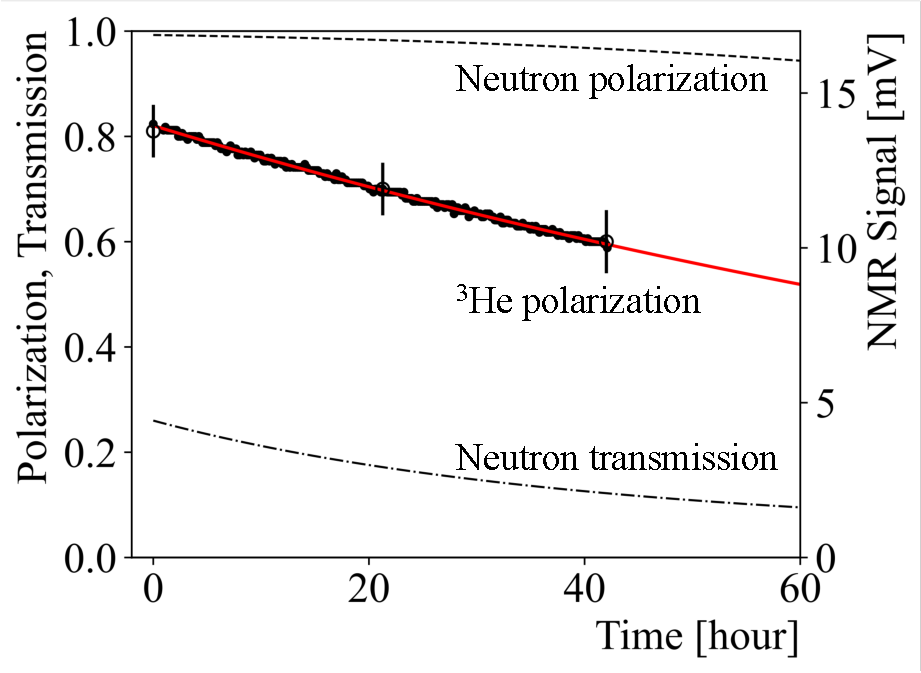
\includegraphics[width=8cm]{figure/NMR_vs_time_20260422.pdf}
%DIFDELCMD <     %%%
%DIFDELCMD < \caption{%
{%DIFAUXCMD
\DIFdelFL{Time dependence of the \He polarization, neutron polarization, and neutron transmission.
    The open circles show the \He polarization obtained from the intensity of the (102) nuclear Bragg peak, while the closed circles show the NMR signal of \He.
    The red line represents the fitting result using an exponential decay function.
    The dashed line indicates the calculated neutron polarization, and the dot-dashed line indicates the calculated neutron transmission.}}
    %DIFAUXCMD
\DIFdelendFL \label{fig:pol_trans_decay}
\end{figure}
\DIFdelbegin %DIFDELCMD < 

%DIFDELCMD < %%%
\DIFdelend \begin{figure}[h]
    \centering
    \DIFdelbeginFL %DIFDELCMD < 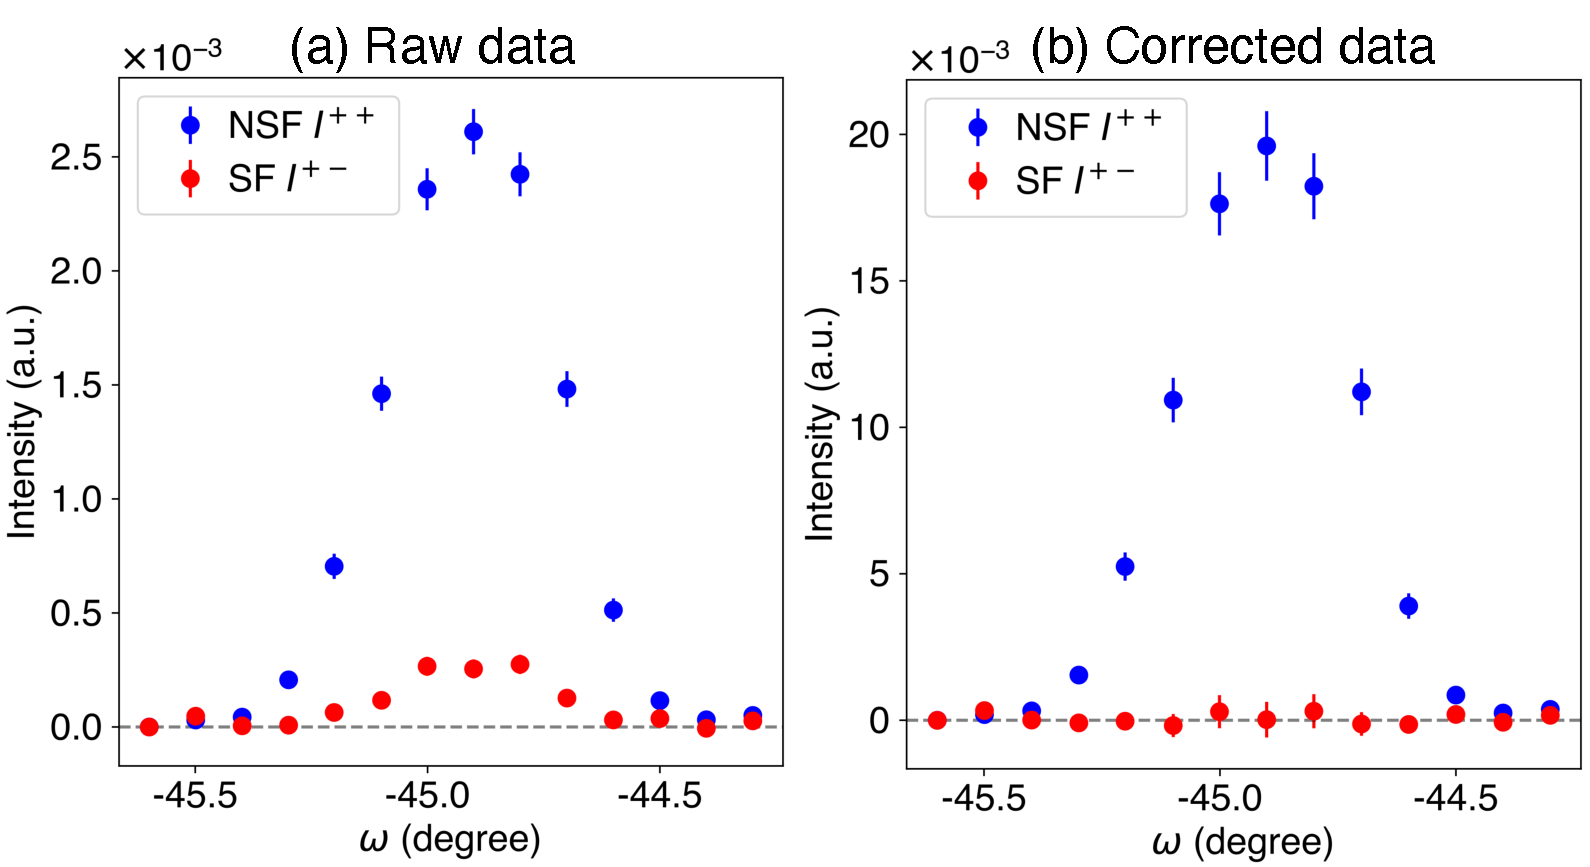
\includegraphics[width=8.5cm]{figure/Polarization_correction_v3.pdf}
%DIFDELCMD <     %%%
\DIFdelendFL \DIFaddbeginFL 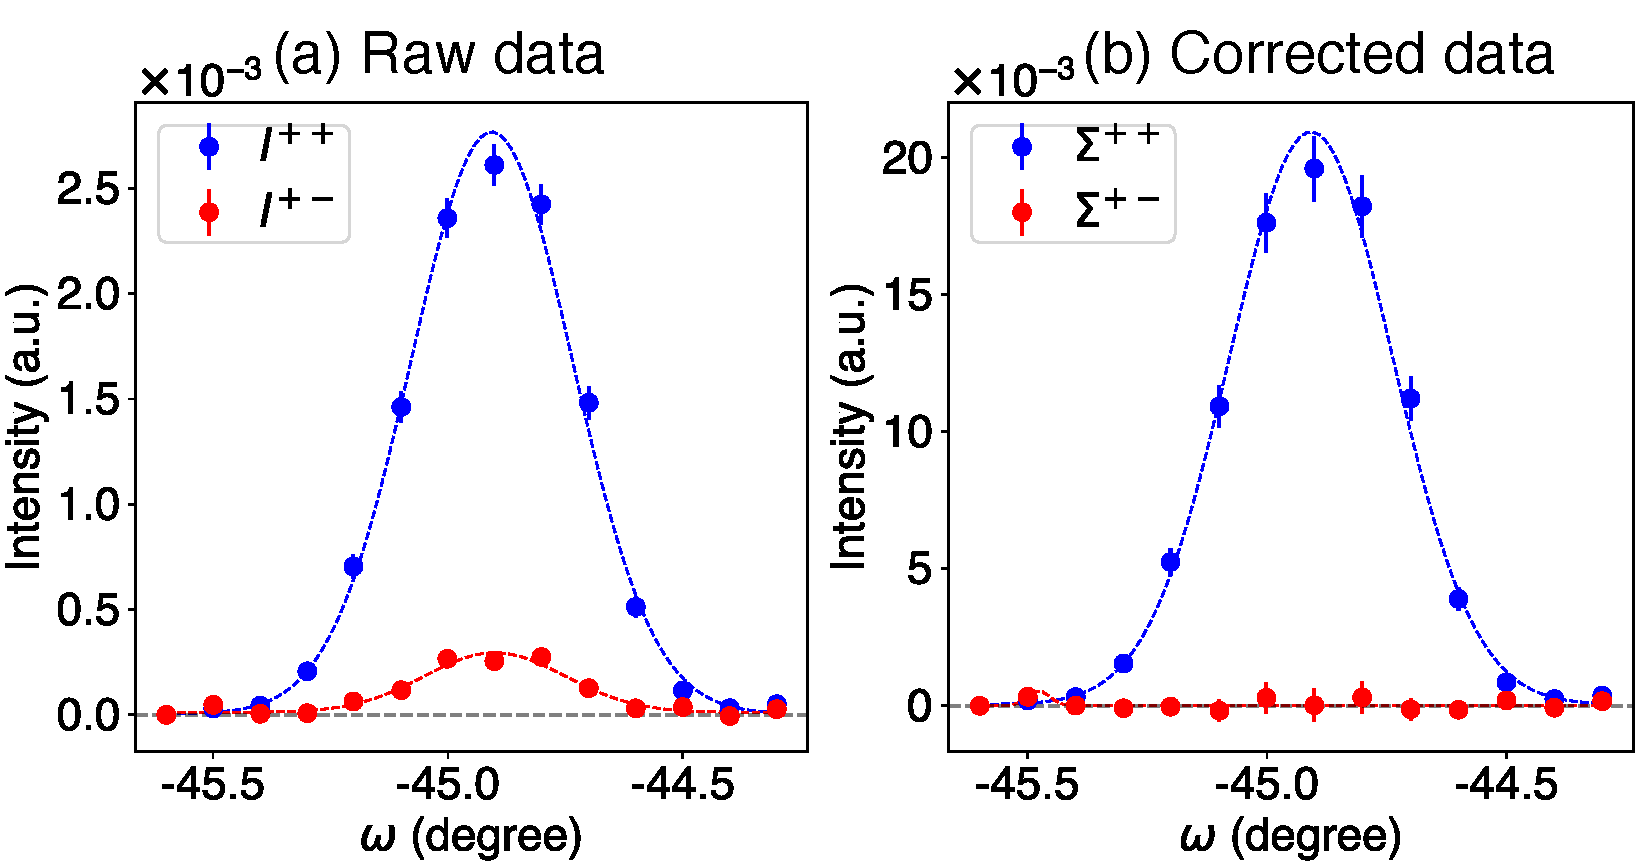
\includegraphics[width=\columnwidth]{figure/Polarization_correction_v4.pdf}
    \DIFaddendFL \caption{\DIFdelbeginFL \DIFdelFL{Intensity }\DIFdelendFL \DIFaddbeginFL \DIFaddFL{The measured intensity }\DIFaddendFL of the \DIFdelbeginFL \DIFdelFL{$(10\bar{2})$ }\DIFdelendFL \DIFaddbeginFL \DIFaddFL{$\bar{1}02$ }\DIFaddendFL reflection \DIFdelbeginFL \DIFdelFL{measured }\DIFdelendFL \DIFaddbeginFL \DIFaddFL{integrated over the peak region identified on the two-dimensional detector }\DIFaddendFL while scanning the sample rotation angle $\omega$.
    \DIFdelbeginFL \DIFdelFL{The red one shows }\DIFdelendFL \DIFaddbeginFL \DIFaddFL{(a) Raw data, where }\DIFaddendFL the \DIFdelbeginFL \DIFdelFL{$I^{++}$ }\DIFdelendFL \DIFaddbeginFL \DIFaddFL{red }\DIFaddendFL and blue \DIFdelbeginFL \DIFdelFL{one shows }\DIFdelendFL \DIFaddbeginFL \DIFaddFL{symbols represent }\DIFaddendFL the \DIFaddbeginFL \DIFaddFL{non-spin-flip intensity $I^{++}$ and spin-flip intensity }\DIFaddendFL $I^{+-}$\DIFaddbeginFL \DIFaddFL{, respectively}\DIFaddendFL .
    \DIFdelbeginFL \DIFdelFL{The left shows the raw }\DIFdelendFL \DIFaddbeginFL \DIFaddFL{(b) Corrected }\DIFaddendFL data, \DIFaddbeginFL \DIFaddFL{where the red }\DIFaddendFL and \DIFaddbeginFL \DIFaddFL{blue symbols represent }\DIFaddendFL the \DIFdelbeginFL \DIFdelFL{right shows the }\DIFdelendFL corrected \DIFdelbeginFL \DIFdelFL{data}\DIFdelendFL \DIFaddbeginFL \DIFaddFL{non-spin-flip and spin-flip scattering cross sections, $\Sigma^{++}$ and $\Sigma^{+-}$, respectively}\DIFaddendFL .}
    \label{fig:polcorrection}
\end{figure}



\subsection{\DIFdelbegin \DIFdel{Application to polarization }\DIFdelend \DIFaddbegin \DIFadd{Polarization }\DIFaddend analysis of \DIFdelbegin \DIFdel{Mn$_3$WO$_6$}\DIFdelend \DIFaddbegin \DIFadd{magnetic scattering}\DIFaddend }
\begin{figure*}[t]
    \centering
    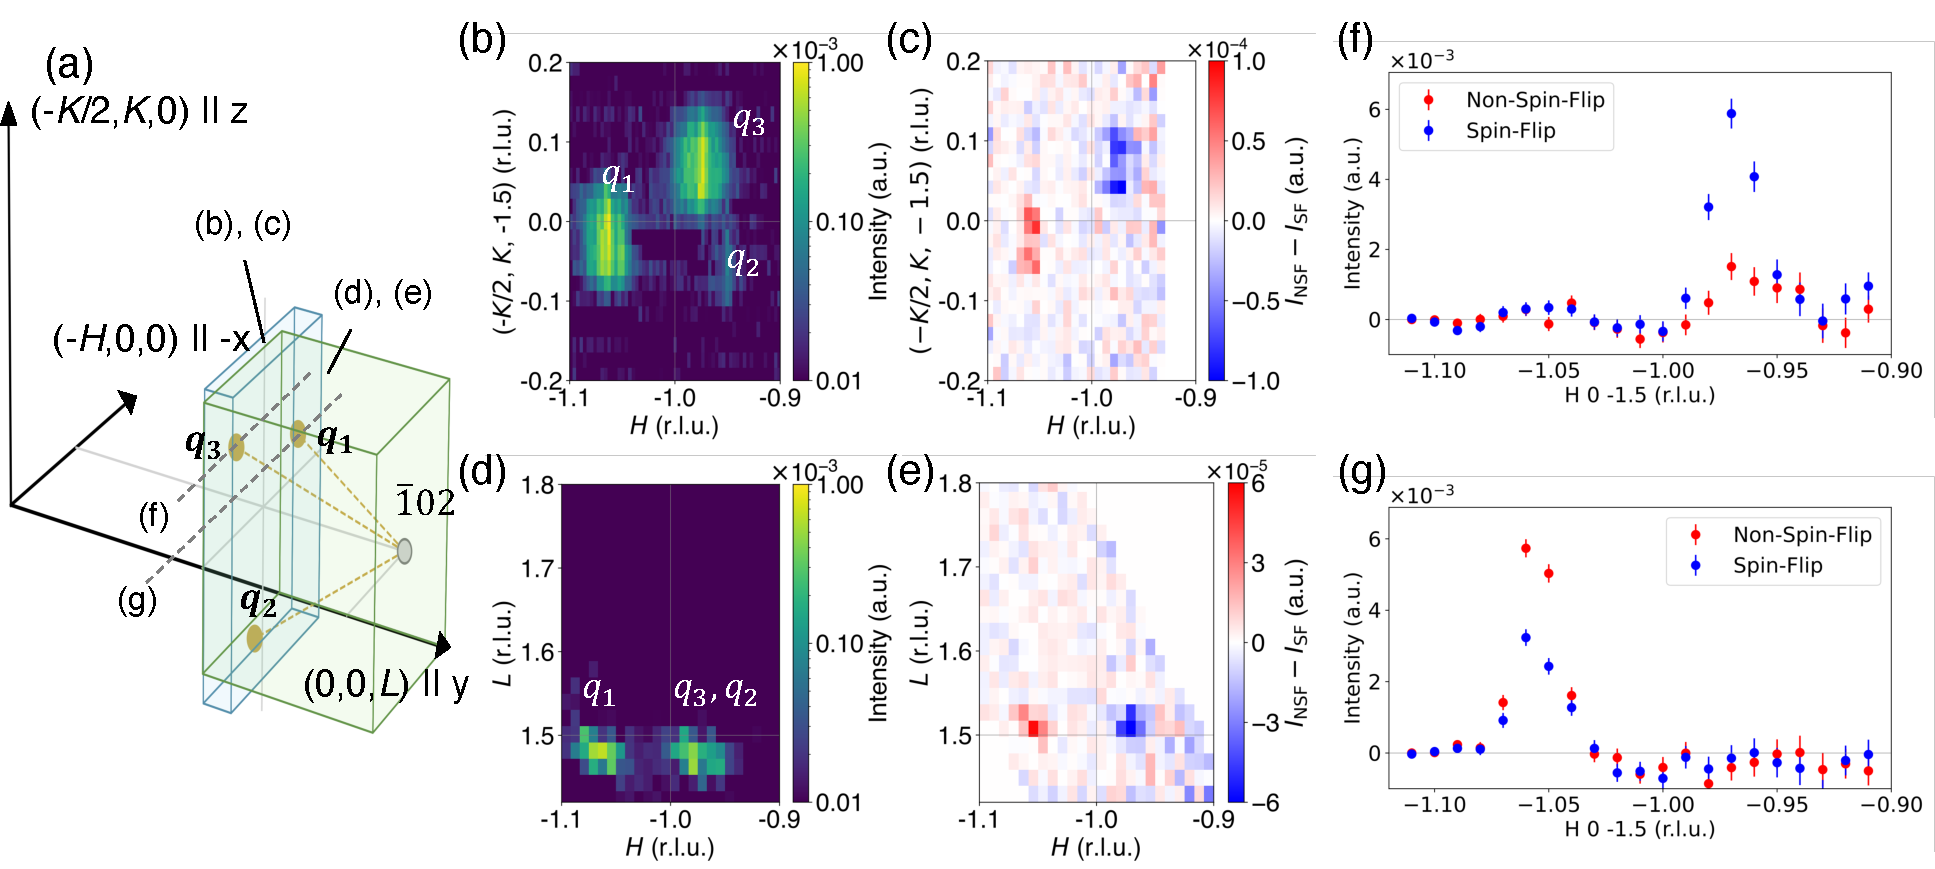
\includegraphics[width=17cm]{figure/Figure6_v4.pdf}
    \caption{
(a) Schematic illustration of the reciprocal-space region measured in the present experiment.
The translucent volumes labeled (b), (c) and (d), (e) indicate the regions integrated along the \(L\) direction and the \((-K/2,K,0)\) direction, respectively.
The dashed lines along the \(-H\) direction through \(\boldsymbol{q}_3\) and \(\boldsymbol{q}_1\) indicate the line cuts shown in panels (f) and (g), respectively.
(b), (d) Unpolarized neutron intensity maps in the \((H,K/2,-1.5)\) and \((H,0,L)\) planes, respectively.
(c), (e) Corresponding polarization-analysis maps obtained from the difference between the non-spin-flip and spin-flip intensities, \(I^{++}-I^{+-}\).
(f), (g) Line profiles of the non-spin-flip and spin-flip intensities at \(\boldsymbol{q}_3\) and \(\boldsymbol{q}_1\), respectively.
}
    \label{fig:measured_Qregion}
\end{figure*}
% 本論文では特に反強磁性転移した23 Kにおける偏極解析結果に焦点をあてて報告する。
\ce{Mn3WO6} is a multiferroic material with a ferroaxial crystal structure belonging to the R$\bar{3}$ space group \cite{maignan_spin-induced_2020}.
This system exhibits successive magnetic phase transitions at T = 25 K and 22.5 K, and spontaneous electric polarization has been reported to appear in the low-temperature magnetically ordered phase.
In this paper, we focus on the polarization analysis results obtained at 23 K, just below the antiferromagnetic transition.
First, using unpolarized neutrons and a two-dimensional detector, intensity maps of antiferromagnetic reflections distributed in the three-dimensional reciprocal space were measured.
This measurement was performed using the setup shown in Fig.~\ref{fig:Setup} without the \Hensf, and the \ce{Cu2MnAl} polarizer was replaced by a PG monochromator.
Figure~\ref{fig:measured_Qregion}(a) shows the reciprocal-space region measured in the present experiment.
Figure~\ref{fig:measured_Qregion}(b) and (d) show intensity maps obtained by integrating the measured intensity along the \(L\) direction and the \((-K/2,K,0)\) direction, respectively.
Because the scattering plane was set to the \((H0L)\) plane, a conventional triple-axis setup would mainly provide a reciprocal-space map in this plane, as shown in Fig.~\ref{fig:measured_Qregion}(d).
In the present experiment, the use of a two-dimensional detector enabled the measured three-dimensional data to be projected along different directions.
In this projection, magnetic reflections characterized by the three propagation vectors \(\boldsymbol{q}_1\), \(\boldsymbol{q}_2\), and \(\boldsymbol{q}_3\) extending from the \(\bar{1}02\) reflection are clearly observed.
Polarized neutron scattering measurements were then performed over the same reciprocal-space regions.
Figures~\ref{fig:measured_Qregion}(c) and \ref{fig:measured_Qregion}(e) show the polarization-analysis maps obtained from the intensity difference \(I^{++}-I^{+-}\).
Clear positive and negative contrasts are observed at the magnetic reflection positions identified in the unpolarized intensity maps.
In addition, to compare the spin-dependent intensities more quantitatively, line profiles along the \(-H\) direction through \(\boldsymbol{q}_3\) and \(\boldsymbol{q}_1\) are shown in Figs.~\ref{fig:measured_Qregion}(f) and \ref{fig:measured_Qregion}(g), respectively.
The relative intensities of the non-spin-flip and spin-flip components are different for the two reflections clearly.
Note that the data in Figs.~\ref{fig:measured_Qregion}(c)-(g) are shown after applying the polarization correction described above.
This indicates that the spin-dependent scattering intensities were successfully resolved for magnetic reflections distributed in three-dimensional reciprocal space.
The polarization-analysis data provide constraints on the magnetic moment components associated with each propagation vector through the relative non-spin-flip and spin-flip intensities.
A detailed magnetic structure analysis based on these constraints will be presented in a separate paper.
% Figure~\ref{fig:measured_Qregion}(d) shows the intensity map obtained by integrating the measured intensity along the \((-K/2,K,0)\) direction.
% This map reveals the distribution of the magnetic reflections along the \(L\) direction, including reflections around \(L\simeq 1.5\), which cannot be fully characterized from the in-plane map alone.
% These unpolarized intensity maps confirm that the magnetic reflections of \ce{Mn3WO6} are distributed over three-dimensional reciprocal space.
% Polarization analysis was then performed for selected magnetic reflections identified from these maps.
% A slice of the measured region taken in the (H0L) plane with $-0.1 \leq K \leq 0.1$ is shown in Fig.~\ref{fig:H0L_HK0_map}(a).
% magnetic reflections are observed at L = -1.5.
% Furthermore, a slice of the measured region in the (H$\frac{K}{2}\bar{1.5}$) plane with $-0.1 \leq L \leq 0.1$ is shown in Fig.~\ref{fig:H0L_HK0_map}(c).
% Several incommensurate magnetic reflections were observed, which were found to correspond to the magnetic propagation vector $\boldsymbol{q} = (0.06, 0.02, 1/2)$ and its threefold rotations about the c axis.
% Polarization analysis was performed for these reflections, and the difference between the non-spin-flip intensity ($I^{++}$) and the spin-flip intensity ($I^{+-}$) is shown in Fig.~\ref{fig:H0L_HK0_map}(b) and (d).
% The incommensurate magnetic reflections corresponding to the threefold rotations exhibit different polarities.
% Furthermore, the intensity profiles obtained by projecting the rectangular regions (e) and (f) in Fig.~\ref{fig:H0L_HK0_map}(d) onto the (H$\frac{K}{2}\bar{1.5}$) axis are shown in Fig.~\ref{fig:H0L_HK0_map}(e) and (f).
% From these results, the present method constrains the symmetry of the magnetic structure and reveals that this phase adopts a collinear sinusoidal magnetic structure.

\section{Summary and Outlook}
In this work, we developed \DIFdelbegin \DIFdel{an experimental approach }\DIFdelend \DIFaddbegin \DIFadd{a polarization analysis method }\DIFaddend that combines a \Hensf~ with a two-dimensional detector to \DIFdelbegin \DIFdel{perform polarization analysis of }\DIFdelend \DIFaddbegin \DIFadd{analyze }\DIFaddend arbitrary reciprocal-lattice points distributed in three-dimensional reciprocal space.
\DIFdelbegin \DIFdel{Although the }\DIFdelend \DIFaddbegin \DIFadd{Polarization analysis was successfully performed for the incommensurate magnetic reflections of \ce{Mn3WO6} at 23 K, and the detail of the magnetic structure will be reported in a separate paper.
The }\DIFaddend positions of the \Hensf~ and the two-dimensional detector were fixed in the present experiment, \DIFdelbegin \DIFdel{polarization analysis of the incommensurate magnetic reflections of \ce{Mn3WO6} at 23 K was successfully performed, leading to the determination of its magnetic structure.
Recently}\DIFdelend \DIFaddbegin \DIFadd{whereas a configuration with both devices mounted on a scanning arm is planned to cover a wider region of reciprocal space.
In addition}\DIFaddend , a compact \textit{in-situ} \Hensf~ system has \DIFaddbegin \DIFadd{recently }\DIFaddend been developed at J-PARC, \DIFdelbegin \DIFdel{where }\DIFdelend \DIFaddbegin \DIFadd{in which }\DIFaddend SEOP is continuously performed during neutron scattering experiments to maintain stable neutron polarization \DIFdelbegin \DIFdel{.
In future experiments, we plan to install both the compact }\textit{\DIFdel{in-situ}} %DIFAUXCMD
\DIFdel{\Hensf~ system and a two-dimensional detector on a scanning arm.
}\DIFdelend \DIFaddbegin \DIFadd{\mbox{%DIFAUXCMD
\cite{takahashi_development_2025}}\hskip0pt%DIFAUXCMD
.
}\DIFaddend This implementation is expected to provide stable neutron polarization during experiments, extend polarization analysis over a wider region of three-dimensional reciprocal space, and contribute to the elucidation of complex magnetic structures in a broader range of materials.
\begin{acknowledgments}
\end{acknowledgments}

\appendix
\section{Polarization correction with \textit{ex-situ} \He neutron spin filter}
\label{appendix}
In this section, the polarization correction \DIFdelbegin \DIFdel{and its error propagation are }\DIFdelend \DIFaddbegin \DIFadd{for measurements using an }\textit{\DIFadd{ex-situ}} \DIFadd{\Hensf~ as an analyzer without a spin flipper is }\DIFaddend described based on the polarization matrix method proposed by A. Wildes \DIFaddbegin \DIFadd{\mbox{%DIFAUXCMD
\cite{wildes_polarizer-analyzer_1999,wildes_scientific_2006}}\hskip0pt%DIFAUXCMD
}\DIFaddend .
The configuration of \DIFdelbegin \DIFdel{the neutron scattering apparatus used }\DIFdelend \DIFaddbegin \DIFadd{apparatus }\DIFaddend in this experiment is shown in Fig.~\ref{fig:appendix}.
The \DIFdelbegin \DIFdel{experiment consists of a polarizer and an analyzer. The spin direction of the }\DIFdelend \DIFaddbegin \DIFadd{spin state of }\DIFaddend incident neutrons polarized by the \ce{Cu2MnAl} single-crystal monochromator is defined as ($+$).
%DIF <  本実験は偏極子、および解析子から構成され、偏極子の\ce{Cu2MnAl}単結晶モノクロメーターが偏極する入射中性子のスピン方向を(+)とする。
\DIFdelbegin \DIFdel{The neutron spin is preserved by a guide magnetic field. The spin }\DIFdelend \DIFaddbegin \DIFadd{The spin }\DIFaddend state of the scattered neutrons \DIFdelbegin \DIFdel{is then }\DIFdelend analyzed by a \Hensf \DIFdelbegin \DIFdel{.
The polarization direction of the \He can be flipped between }\DIFdelend \DIFaddbegin \DIFadd{is defined as}\DIFaddend ($+$) \DIFdelbegin \DIFdel{and }\DIFdelend \DIFaddbegin \DIFadd{or }\DIFaddend ($-$)\DIFdelbegin \DIFdel{using the AFP NMR, and no neutron spin flipper was employed in this experiment}\DIFdelend \DIFaddbegin \DIFadd{, where polarization can be flipped using AFP NMR}\DIFaddend .
When the \Hensf~ is polarized in the ($+$)\DIFdelbegin \DIFdel{direction}\DIFdelend , the neutron intensity measured at the detector consists of four contributions \DIFdelbegin \DIFdel{, }\DIFdelend as illustrated in Fig.~\ref{fig:appendix}\DIFdelbegin \DIFdel{, and can be written as follows.
}\DIFdelend \DIFaddbegin \DIFadd{.
It is expressed as
}\DIFaddend \begin{align}
    I^{++} &= N_0 T_p p_p \Sigma^{++} T_a p_a \notag \\
    &+ N_0 T_p p_p \Sigma^{+-} T_a (1-p_a) \notag\\
    &+N_0 T_p (1-p_p) \Sigma^{-+} T_a p_a \notag \\
    &+ N_0 T_p (1-p_p) \Sigma^{--} T_a (1-p_a)\DIFaddbegin \DIFadd{,
    }\DIFaddend \label{eq:Ipp}
\end{align}
% \begin{align}
% I^{++} &= N_+ T_p^+ p_p^+ \Sigma^{++} T_a^+ p_a^+ \notag \\
% &+ N_+ T_p^+ p_p^+ \Sigma^{+-} T_a^+ (1-p_a^+) \notag\\
% &+N_- T_p^+ (1-p_p^+) \Sigma^{-+} T_a^+ p_a^+ \notag \\
% &+ N_- T_p^+ (1-p_p^+) \Sigma^{--} T_a^+ (1-p_a^+)
% \label{eq:Ipp}
% \end{align}
where $N_0$ is the number of incident neutrons,
$T_p$ \DIFdelbegin \DIFdel{,}\DIFdelend \DIFaddbegin \DIFadd{and }\DIFaddend $T_a$ are the total neutron \DIFdelbegin \DIFdel{transmission }\DIFdelend \DIFaddbegin \DIFadd{transmissions }\DIFaddend of the polarizer and analyzer,
$p_p$ and $p_a$ are the polarization \DIFdelbegin \DIFdel{efficiency }\DIFdelend \DIFaddbegin \DIFadd{efficiencies }\DIFaddend of the polarizer and analyzer,
$\Sigma^{++}$, $\Sigma^{+-}$, $\Sigma^{-+}$, and $\Sigma^{--}$ are the scattering cross sections for the corresponding spin states.
The polarization \DIFdelbegin \DIFdel{efficiency }\DIFdelend \DIFaddbegin \DIFadd{efficiencies, }\DIFaddend $p_p$ and $p_a$ are defined \DIFdelbegin \DIFdel{in the range 0.5 $\leq$ $p_p$, $p_a$ $\leq$ 1, and their }\DIFdelend \DIFaddbegin \DIFadd{as $0.5 \leq p_p \leq 1$ and $0.5 \leq p_a \leq 1$, respectively.
Their }\DIFaddend relation to the neutron polarization is given by $P_p = 2p_p -1$ and $P_a = 2p_a -1$.
%DIF <  中性子偏極度との関係は$P_p = 2p_p -1$、$P_a = 2p_a -1$で表される。
%DIF <  本実験のセットアップから測定可能な条件は$I^{++}$と$I^{+-}$の2つであり、
%DIF <  Assuming that the numbers of incident neutrons with spin ($+$) and ($-$) from the reactor neutron source are equalとすると式\ref{eq:I_pp}は以下の行列式で簡略化できる。
\begin{figure}[t]
    \centering
    \DIFdelbeginFL %DIFDELCMD < 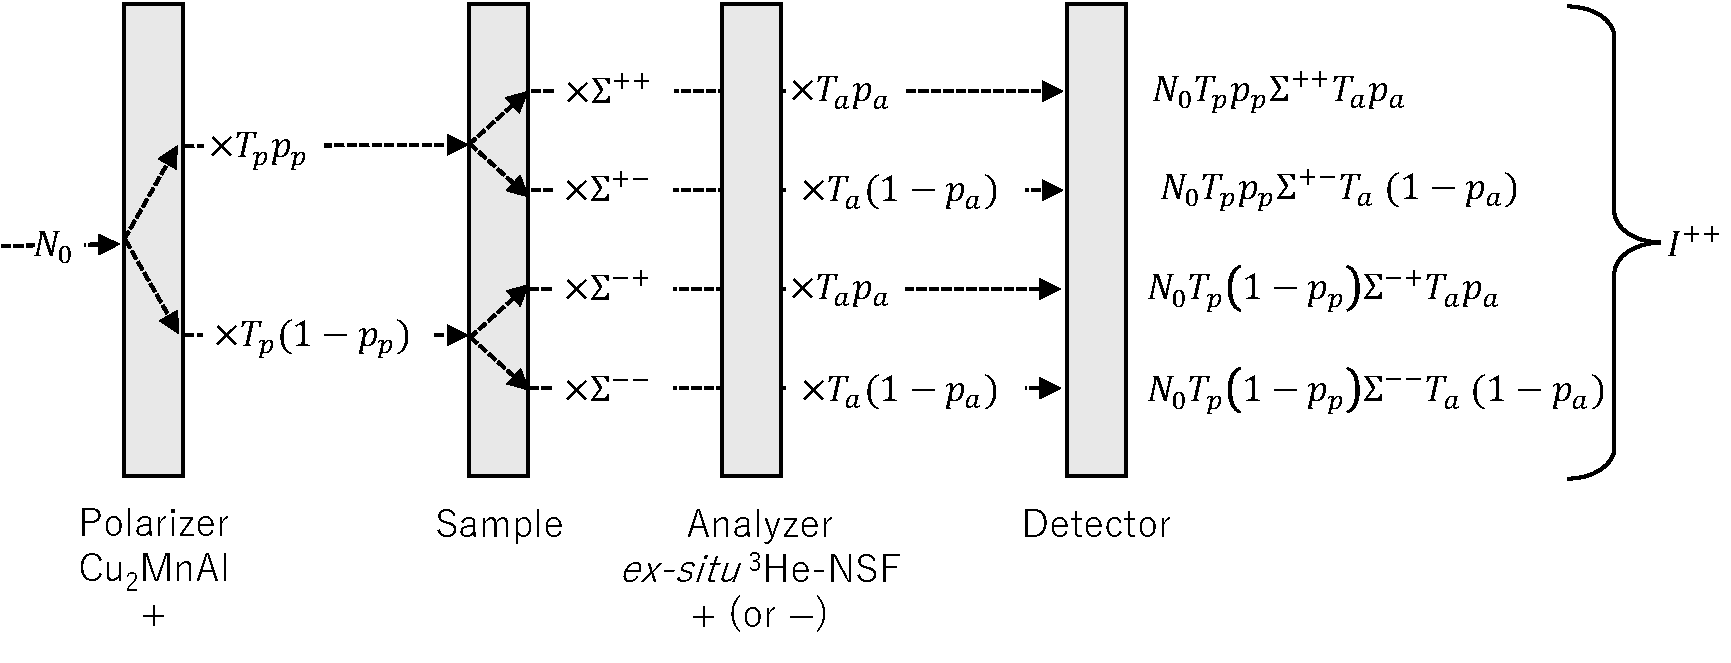
\includegraphics[width=8.5cm]{figure/Appendix_v5.pdf}
%DIFDELCMD <     %%%
\DIFdelendFL \DIFaddbeginFL 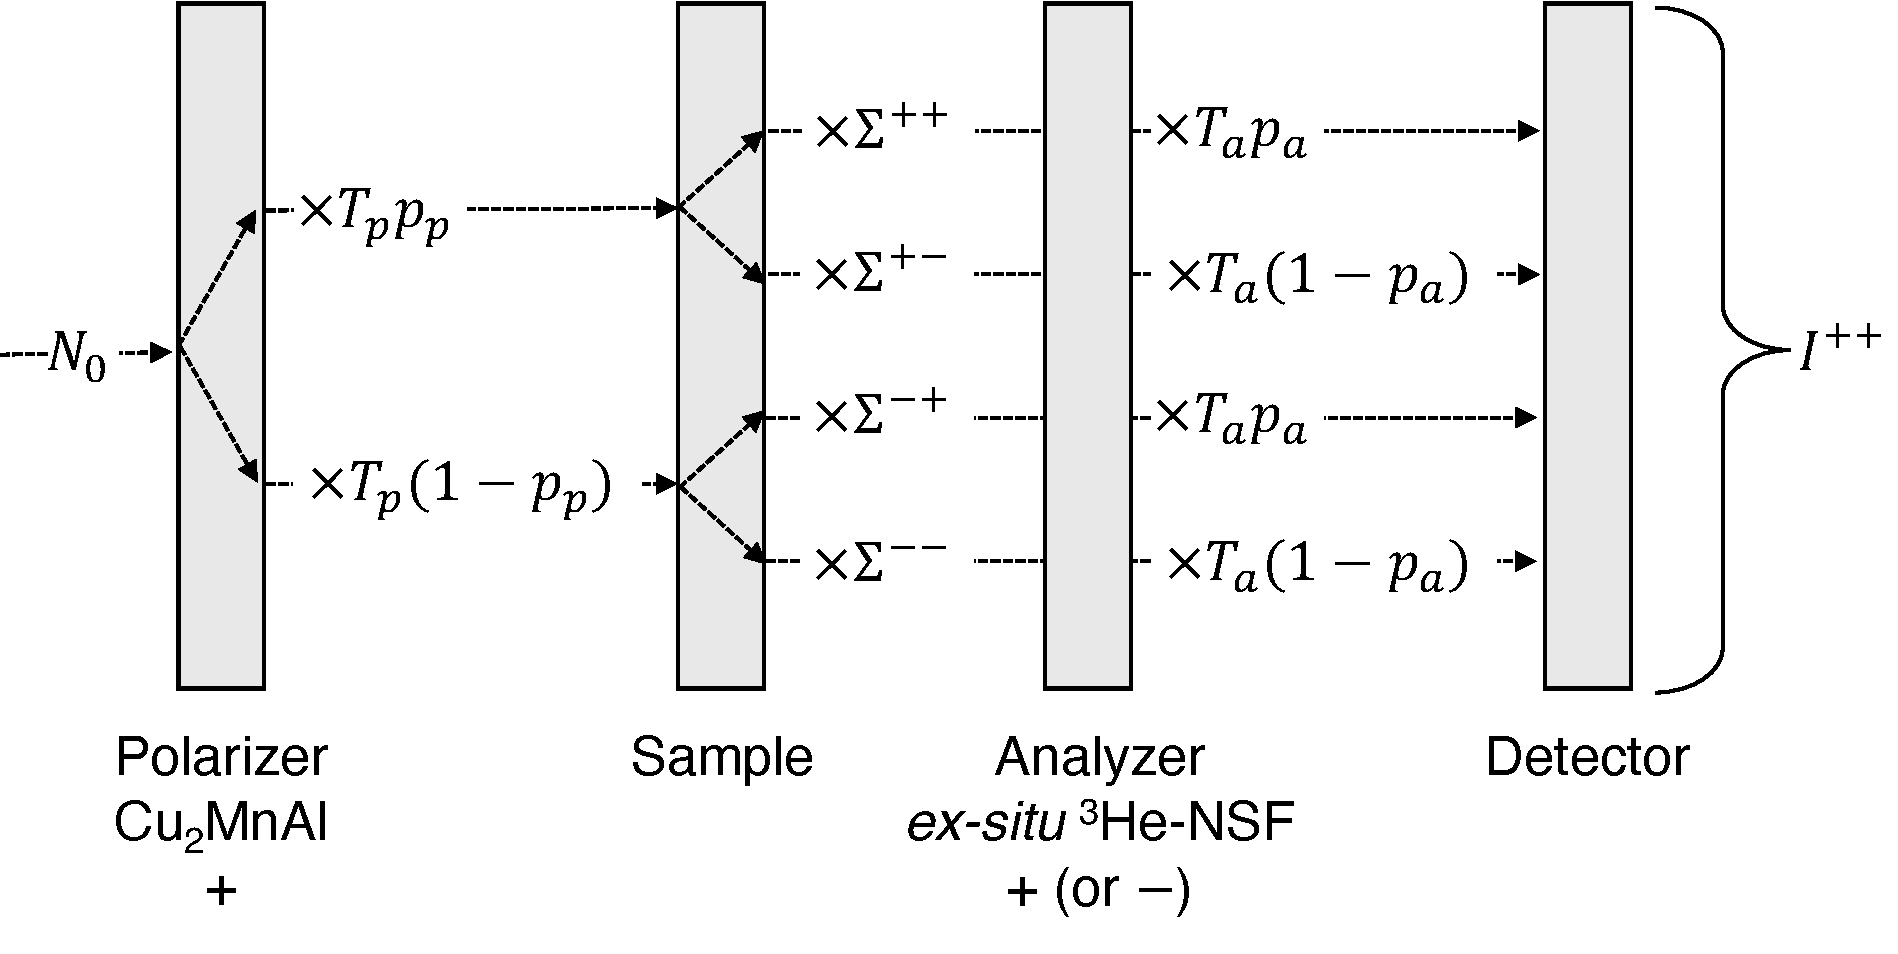
\includegraphics[width=8.5cm]{figure/Appendix_v6.pdf}
    \DIFaddendFL \caption{Schematic diagram of the spin-dependent neutron intensity in the polarized neutron scattering experiment.
    The incident beam with intensity $N_0$ is polarized by the \ce{Cu2MnAl} polarizer and then scattered by the sample with the spin-dependent cross sections $\Sigma^{++}$, $\Sigma^{+-}$, $\Sigma^{-+}$, and $\Sigma^{--}$.
    The scattered neutrons are analyzed by the \DIFdelbeginFL \textit{\DIFdelFL{ex-situ}} %DIFAUXCMD
\DIFdelendFL \Hensf~ with transmission $T_a$ and polarization \DIFaddbeginFL \DIFaddFL{efficiency }\DIFaddendFL $p_a$\DIFdelbeginFL \DIFdelFL{before being detected}\DIFdelendFL .
    The \DIFdelbeginFL \DIFdelFL{detected }\DIFdelendFL \DIFaddbeginFL \DIFaddFL{measured }\DIFaddendFL intensity $I^{++}$ is given by the sum of the contributions from the four spin-scattering channels when \ce{Cu2MnAl} and \Hensf~ are both polarized in the same direction.}
    \label{fig:appendix}
\end{figure}
Only two configurations, $I^{++}$ and $I^{+-}$ can be measured in this experimental setup.
Assuming that the numbers of incident neutrons with spin ($+$) and ($-$) from the reactor neutron source are equal \DIFaddbegin \DIFadd{and that the scattering cross sections satisfy $\Sigma^{++} = \Sigma^{--}$ and $\Sigma^{+-} = \Sigma^{-+}$}\DIFaddend ,
Eq.~\ref{eq:Ipp} can be \DIFdelbegin \DIFdel{simplified into }\DIFdelend \DIFaddbegin \DIFadd{rewritten in }\DIFaddend the following matrix form:
\begin{widetext}
    \begin{align}
        \begin{bmatrix}
            I^{++} \\
            I^{+-}
        \end{bmatrix}
        =
        \begin{bmatrix}
            T_p p_p T_a p_a + T_p (1-p_p) T_a (1-p_a) & T_p p_p T_a (1-p_a) + T_p (1-p_p) T_a p_a \\
            T_p p_p T_a (1-p_a) + T_p (1-p_p) T_a p_a & T_p p_p T_a p_a + T_p (1-p_p) T_a (1-p_a) \\
        \end{bmatrix}
        \begin{bmatrix}
            \Sigma^{++} \\
            \Sigma^{+-}
        \end{bmatrix}\DIFaddbegin \DIFadd{,
        }\DIFaddend \label{eq:Ipp_Ipm}
    \end{align}
\end{widetext}
%DIF <  \textit{ex-situ} \Hensfは時間経過とともに\He 偏極度が減衰するため、中性子偏極能率や透過率も時間依存することから、上式の行列要素も時間依存したものとなる。
%DIF <  そのため、式\ref{eq:Ipp_Ipm}行列要素を時間依存するものとして表しを逆行列をとると以下のようになる。
Since the \textit{ex-situ} \Hensf~ exhibits a decay of the \He polarization over time, both the neutron polarization efficiency $p_a$ and the neutron transmission $T_a$ become time dependent.
% the above expression can be written in matrix form for the cases where the polarizer and analyzer are set to ($+$) and ($-$), respectively, as follows:
Accordingly, by treating Eq.~\ref{eq:Ipp_Ipm} as a time-dependent matrix equation and taking its inverse, the following expression is obtained\DIFdelbegin \DIFdel{.
}\DIFdelend \DIFaddbegin \DIFadd{:
}\DIFaddend \begin{widetext}
    \begin{align}
        \begin{bmatrix}
            \Sigma^{++} \\
            \Sigma^{+-}
        \end{bmatrix}
        &=\DIFdelbegin \DIFdel{\frac{1}{T_p^2 T_a(t_1) T_a(t_2) (2p_p -1)(p_a(t_1)+p_a(t_2) -1)} \times }%DIFDELCMD < \notag\\
%DIFDELCMD <         %%%
%DIF <  \frac{1}{}
        %DIFDELCMD < &\begin{bmatrix}
%DIFDELCMD <             T_p T_a(t_2) (p_p p_a(t_2) + (1-p_p)(1-p_a(t_2))) & -T_p T_a(t_1) (p_p (1-p_a(t_1)) + (1-p_p) p_a(t_1)) \\
%DIFDELCMD <             -T_p T_a(t_2) (p_p (1-p_a(t_2)) + (1-p_p) p_a(t_2)) & T_p T_a(t_1) (p_p p_a(t_1) + (1-p_p)(1-p_a(t_1))) \\
%DIFDELCMD <         \end{bmatrix}
%DIFDELCMD <         \begin{bmatrix}
%DIFDELCMD <             I^{++}(t_1) \\
%DIFDELCMD <             I^{+-}(t_2)
%DIFDELCMD <         \end{bmatrix}
%DIFDELCMD <         \notag\\
%DIFDELCMD <         &%%%
\DIFdel{=}\DIFdelend \frac{1}{T_p^2T_a(t_1)T_a(t_2)P_p(P_a(t_1)+P_a(t_2))}
        \begin{bmatrix}
            T_pT_a(t_2)(1+P_pP_a(t_2)) & -T_pT_a(t_1)(1-P_pP_a(t_1)) \\
            -T_pT_a(t_2)(1-P_pP_a(t_2)) & T_pT_a(t_1)(1+P_pP_a(t_1)) \\
\end{bmatrix}
\begin{bmatrix}
    I^{++}(t_1) \\
    I^{+-}(t_2)
\end{bmatrix}\DIFaddbegin \DIFadd{,
}\DIFaddend \label{eq:Sigma}
\end{align}
\end{widetext}
\DIFdelbegin %DIFDELCMD < 

%DIFDELCMD < %%%
%DIF <  改めて\Hensf~における\He 偏極度と中性子透過率$T$と中性子偏極度$P$は以下の式で表される。
\DIFdel{The \He polarization $P_\mathrm{He}$, the neutron transmission $T$, and the neutron polarization $P$ in the \Hensf~ are given by the following expressions.
%DIF <  \begin{align}
%DIF <      P_{\mathrm{He}}(t) &= P_{\mathrm{He}}(t_0) \exp(-t/\tau), \\
%DIF <      T(t) &= \exp(-\rho d \sigma(\lambda)) \cosh(\rho d \sigma(\lambda) P_{\mathrm{He}}(t)). \\
%DIF <      P(t) &= \tanh(\rho d \sigma(\lambda) P_{\mathrm{He}}(t)).
%DIF <  \end{align}
%DIF <  これらを実験的に求めて式\ref{eq:Sigma}に代入することで、偏極補正された散乱強度を得た。
These quantities are experimentally determined }\DIFdelend \DIFaddbegin \DIFadd{where $p_p$ and $p_a$ are transformed into $P_p$ }\DIFaddend and \DIFdelbegin \DIFdel{substituted into Eq. ~\ref{eq:Sigma}.
%DIF <  図\ref{fig:polcorrection}は、実験で得られた$T_a$,$P_a$を用いて偏極補正を行った$(10\bar{2})$の結果を示す。
%DIF <  ここで、\ce{Cu2MnAl}単結晶モノクロメーターの中性子透過率$T_p$は定数であるため入射中性子フラックスに押し込み、
%DIF <  中性子偏極度$P_p$はピークトップ時の$\omega = 44.9^{\circ}$における核反射($10\bar{2}$)強度から求めた。
%DIF <  補正後の図はNon-spin flip scatteringの強度が増加し、Spin flip scatteringの強度が減少していることがわかる。
%DIF <  これは時間経過とともに減少する中性子透過率中性子偏極度がうまく補正されていることを示している。
Figure \ref{fig:polcorrection} shows the $(10\bar{2})$ reflection intensities at $I^{++}$}\DIFdelend \DIFaddbegin \DIFadd{$P_a$ using the relation described above.
The experimentally determined values of $T_a(t)$}\DIFaddend , \DIFdelbegin \DIFdel{$I^{+-}$ and the results after applying the polarization correction using the experimentally obtained $T_a$ and $P_a$.
%DIF <  Since the neutron transmission of the \ce{Cu2MnAl} single-crystal monochromator, $T_p$, is constant, it was incorporated into the incident neutron flux.
The constant neutron transmission }\DIFdelend \DIFaddbegin \DIFadd{$P_p$, and $P_a(t)$ are described in the Sec. \ref{sec:He-3}.
While $T_a(t)$ and $P_a(t)$ vary with time owing to the relaxation of the \He polarization, }\DIFaddend $T_p$ \DIFdelbegin \DIFdel{of the \ce{Cu2MnAl} single-crystal monochromator was absorbed into the incident neutron flux.
The non-spin-flip scattering intensity increases while the }\DIFdelend \DIFaddbegin \DIFadd{is constant throughout the measurement.
Therefore, $T_p$ only gives a common scale factor to the scattering cross sections.
Thus, these polarization correction yields the non-spin-flip and }\DIFaddend spin-flip scattering \DIFdelbegin \DIFdel{intensity decreases after the correction.
These results indicate that the time-dependent decrease in neutron transmission and neutron polarization of \Hensf~ are properly corrected.
}%DIFDELCMD < 

%DIFDELCMD < %%%
%DIF <  原子炉中性子源からでてくる中性子数は$N_+$と$N_-$が等しいとすると、上式はpolarizerとanalyzerが+と-それぞれの場合について、以下のように行列形式で表すことができる。
%DIF <  中性子スピンはガイド磁場によって維持され、試料で散乱された後、\Hensf~によって解析される。
%DIF <  このとき、\Hensf~はAFP NMR法を用いることで、\He の極性を(+)と(-)と切り替えることが可能であり、中性子スピンフリッパーは用いていない。
%DIF <  \Hensf~が(+)方向に偏極しているときに検出器に到達する中性子強度は図\ref{fig:appendix}中に表されるように4つの項から成り、以下で表される。
%DIFDELCMD < 

%DIFDELCMD < %%%
%DIF <  \begin{equation}
%DIF <  \begin{bmatrix}
%DIF <  I^{00}(t_1) \\
%DIF <  I^{01}(t_2)
%DIF <  \end{bmatrix}
%DIF <  =
%DIF <  \begin{bmatrix}
%DIF <  R_ppR_a(t_1)a(t_1)+R_p(1-p)R_a(t_1)(1-a(t_1)) & R_ppR_a(t_1)(1-a(t_1))+R_p(1-p)R_a(t_1)a(t_1)\\
%DIF <  R_ppR_a(t_2)(1-a(t_2))+R_p(1-p)R_a(t_2)a(t_2) & R_ppR_a(t_2)a(t_2)+R_p(1-p)R_a(t_2)(1-a(t_2))\\
%DIF <  \end{bmatrix}
%DIF <  \begin{bmatrix}
%DIF <  \Sigma^{++} \\
%DIF <  \Sigma^{+-}
%DIF <  \end{bmatrix}
%DIF <  \end{equation}
\DIFdelend \DIFaddbegin \DIFadd{cross sections, $\Sigma^{++}$ and $\Sigma^{+-}$.
}\DIFaddend 





\bibliographystyle{apsrev4-2}
\bibliography{ref}

\end{document}
%
% ****** End of file apssamp.tex ******
